% The use of oneside here is a temporary hack; \marginpar entries
% don't show up on odd pages of PDF output without it.  Sigh.
%\documentclass[oneside]{book}
%\documentclass[landscape]{book}
%\documentclass[a5paper]{book}
\documentclass[letterpaper]{book}

\usepackage{enumerate}
\usepackage{fullpage}
\usepackage{makeidx}
\usepackage{ifpdf}
\usepackage{graphicx}
\usepackage{pslatex}
\usepackage{fancyvrb}
% source code listing
\usepackage{listings}
% to find out he layout
% \usepackage{layouts}

%\evensidemargin=25pt
%\oddsidemargin=25pt
% hobbit source code is quite wide,6.5in is not wide engough.
\setlength{\textwidth}{7.1in}
\addtolength{\voffset}{-5pt}



% leave hyperref until last
\usepackage[colorlinks=true,bookmarks=true,pdftitle={Distributed
  revision control with Mercurial},pdfsubject={Revision
  control},pdfkeywords={Mercurial, Revision control, Distributed
  revision control},pdfauthor={Tyng-Jing Yang}]{hyperref}


% This file is a collection latex custom commands created for this book.

% Mercurial command.
\newcommand{\hbgraph}[1]{\index{\texttt{#1} hobbit graph}``\texttt{hg #1}''}

%
% Bug ID.
\newcommand{\bug}[1]{\index{Mercurial bug
    database!\href{http://www.selenic.com/mercurial/bts/issue#1}{bug
      ~#1}}\href{http://www.selenic.com/mercurial/bts/issue#1}{Mercurial
    bug no.~#1}}

% File name in the user's home directory.
\newcommand{\tildefile}[1]{\texttt{\~{}/#1}}

% File name.
\newcommand{\filename}[1]{\texttt{#1}}

% Directory name.
\newcommand{\dirname}[1]{\texttt{#1}}

% File name, with index entry.
% The ``s'' prefix comes from ``special''.
\newcommand{\sfilename}[1]{\index{\texttt{#1} file}\texttt{#1}}

% Directory name, with index entry.
\newcommand{\sdirname}[1]{\index{\texttt{#1} directory}\texttt{#1}}

% Mercurial extension.
\newcommand{\hgext}[1]{\index{\texttt{#1} extension}\texttt{#1}}

% Command provided by a Mercurial extension.
\newcommand{\hgxcmd}[2]{\index{\texttt{#2} command (\texttt{#1}
      extension)}\index{\texttt{#1} extension!\texttt{#2} command}``\texttt{hg #2}''}

% Mercurial command.
\newcommand{\hgcmd}[1]{\index{\texttt{#1} command}``\texttt{hg #1}''}

%%%%%%%%%%%%%%%%%%%%%%%%%%%%%%%%%%%%%%%%%%%%
% Definition for MOTO Hobbit.
%%%%%%%%%%%%%%%%%%%%%%%%%%%%%%%%%%%%%%%%%%%%
\newcommand{\motohbcmd}[1]{\index{\texttt{#1} command}``\texttt{/opt/bin/#1}''}
\newcommand{\motoserverconfig}[1]{\index{\texttt{#1} command}``\texttt{/etc/opt/hobbitserver42/#1}''}

% Mercurial command, with arguments.
\newcommand{\hgcmdargs}[2]{\index{\texttt{#1} command}``\texttt{hg #1 #2}''}
\newcommand{\tplkword}[1]{\index{\texttt{#1} template keyword}\index{template keywords!\texttt{#1}}\texttt{#1}}
\newcommand{\tplkwfilt}[2]{\index{\texttt{#1} template keyword!\texttt{#2}
    filter}\index{template filters!\texttt{#2}}\index{\texttt{#2}
    template filter}\texttt{#2}}

\newcommand{\tplfilter}[1]{\index{template
    filters!\texttt{#1}}\index{\texttt{#1} template
    filter}\texttt{#1}}

% Shell/system command.
\newcommand{\command}[1]{\index{\texttt{#1} system command}\texttt{#1}}

% Shell/system command, with arguments.
\newcommand{\cmdargs}[2]{\index{\texttt{#1} system command}``\texttt{#1 #2}''}

% Mercurial command option.
\newcommand{\hgopt}[2]{\index{\texttt{#1} command!\texttt{#2} option}\texttt{#2}}

% Mercurial command option, provided by an extension command.
\newcommand{\hgxopt}[3]{\index{\texttt{#2} command (\texttt{#1} extension)!\texttt{#3} option}\index{\texttt{#1} extension!\texttt{#2} command!\texttt{#3} option}\texttt{#3}}

% Mercurial global option.
\newcommand{\hggopt}[1]{\index{global options!\texttt{#1} option}\texttt{#1}}

% Shell/system command option.
\newcommand{\cmdopt}[2]{\index{\texttt{#1} command!\texttt{#2} option}\texttt{#2}}

% Command option.
\newcommand{\option}[1]{\texttt{#1}}

% Software package.
\newcommand{\package}[1]{\index{\texttt{#1} package}\texttt{#1}}

% Section name from a hgrc file.
\newcommand{\rcsection}[1]{\index{\texttt{hgrc} file!\texttt{#1} section}\texttt{[#1]}}

% Named item in a hgrc file section.
\newcommand{\rcitem}[2]{\index{\texttt{hgrc} file!\texttt{#1}
    section!\texttt{#2} entry}\texttt{#2}}

% hgrc file.
\newcommand{\hgrc}{\index{configuration file!\texttt{hgrc}
    (Linux/Unix)}\index{\texttt{hgrc} configuration file}\texttt{hgrc}}

% Mercurial.ini file.
\newcommand{\hgini}{\index{configuration file!\texttt{Mercurial.ini}
    (Windows)}\index{\texttt{Mercurial.ini} configuration file}\texttt{Mercurial.ini}}

% Hook name.
\newcommand{\hook}[1]{\index{\texttt{#1} hook}\index{hooks!\texttt{#1}}\texttt{#1}}

% Environment variable.
\newcommand{\envar}[1]{\index{\texttt{#1} environment
    variable}\index{environment variables!\texttt{#1}}\texttt{#1}}

% Python module.
\newcommand{\pymod}[1]{\index{\texttt{#1} module}\texttt{#1}}

% Python class in a module.
\newcommand{\pymodclass}[2]{\index{\texttt{#1} module!\texttt{#2}
    class}\texttt{#1.#2}}

% Python function in a module.
\newcommand{\pymodfunc}[2]{\index{\texttt{#1} module!\texttt{#2}
    function}\texttt{#1.#2}}

% Note: blah blah.
\newsavebox{\notebox}
\newenvironment{note}%
  {\begin{lrbox}{\notebox}\begin{minipage}{0.7\textwidth}\textbf{Note:}\space}%
  {\end{minipage}\end{lrbox}\fbox{\usebox{\notebox}}}
\newenvironment{caution}%
  {\begin{lrbox}{\notebox}\begin{minipage}{0.7\textwidth}\textbf{Caution:}\space}%
  {\end{minipage}\end{lrbox}\fbox{\usebox{\notebox}}}

% Code sample, eating 4 characters of leading space.
\DefineVerbatimEnvironment{codesample4}{Verbatim}{frame=single,gobble=4,numbers=left,commandchars=\\\{\}}

% Code sample, eating 2 characters of leading space.
\DefineVerbatimEnvironment{codesample2}{Verbatim}{frame=single,gobble=2,numbers=left,commandchars=\\\{\}}

% Interaction from the examples directory.
\newcommand{\interaction}[1]{\VerbatimInput[frame=single,numbers=left,commandchars=\\\{\}]{examples/#1.lxo}}
% Example code from the examples directory.
\newcommand{\excode}[1]{\VerbatimInput[frame=single,numbers=left,commandchars=\\\{\}]{../examples/#1}}

% Graphics inclusion.
\ifpdf
  \newcommand{\grafix}[1]{\includegraphics{#1}}
\else
  \newcommand{\grafix}[1]{\includegraphics{#1.png}}
\fi

% Reference entry for a command.
\newcommand{\cmdref}[2]{\section{\hgcmd{#1}---#2}\label{cmdref:#1}\index{\texttt{#1} command}}

% Reference entry for a command option with long and short forms.
\newcommand{\optref}[3]{\subsubsection{\hgopt{#1}{--#3}, also \hgopt{#1}{-#2}}}

% Reference entry for a command option with only long form.
\newcommand{\loptref}[2]{\subsubsection{\hgopt{#1}{--#2} option}}

%%% Local Variables: 
%%% mode: latex
%%% TeX-master: "00book"
%%% End: 


\title{System Monitoring with Hobbit: Source Codes } \author{T.J. Yang}
\date{Copyright \copyright\ 2008 Tyng-Jing Yang.\\
  This material may be distributed only subject to the terms and
  conditions set forth in version 1.0 of the Open Publication License.
  Please refer to Appendix~\ref{cha:opl} for the license text.\\
  This book was prepared from
  \href{http://hg.serpentine.com/mercurial/book/}{rev~c9202b05c4f5, dated 2008-01-29 17:34 -0600,}
  using \href{http://www.selenic.com/hg/}{rev~Mercurial Distributed SCM (version 0.9.3)}.
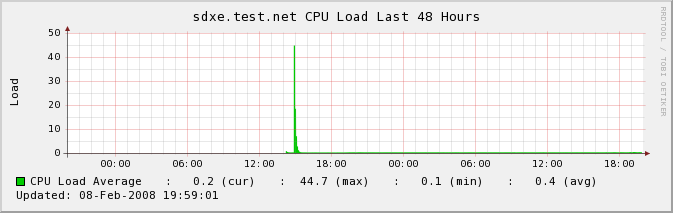
\includegraphics[scale=0.5]{./hobbitgraph.png} 
}

\makeindex

\begin{document}


\maketitle

\addcontentsline{toc}{chapter}{Contents}
\pagenumbering{roman}
\tableofcontents
\listoffigures
%\listoftables

\pagenumbering{arabic}

\chapter{Preface}
\label{chap:preface}



\section{Skill set  Requirements }
There are a few requirements in order for you to particpate in
hobbitmon developement.

But if you don't have these skills currently, that is fine. If you
study hard with this book. You will gain all these skills once you
finish reading this book.


\begin{itemize}
\item You are doing this for free.
\item You are doing this for free without direct pay from the
  community. And to this date not many people can make money directly.

\item Ok, you have been warned. The first requirement is C programming
  language. but it doesn't stop here only at C language. There are
  many other language like Perl, Python and shell language used to
  develop modules. 
\item subversion source code management system.
\item GNU Make.
\item GNU Autotool.
\item GNU TWW CPAM tool.
\item Latex.
\item Doxygen.
\item Editor. Emacs preferred ;)
 
\end{itemize}

\section{This book is a work in progress}

I am writing this  book about hobbit from perspective of manpages.  

I am releasing this Hobbit RTFM book while I am still writing it, in the hope that
it will prove useful to others.  I also hope that readers will contribute as they see fit.

\section{Hobbit Documentation Road Map}


\begin{itemize}
\item Hobbit RTFM.
\item Hobbit User Guide.
\item Hobbit Developer Guide.
\item Hobbit Administration Guide.
\item Hobbit Slides.

\end{itemize}

\section{Revision History}

\begin{itemize}
\item Henrik Storner
 \begin{enumerate}
  \item Wrote the orignial manpages in troff format.
 \end{enumerate}

\item T.J. Yang:
 \begin{enumerate}
  \item Import from troff source files to LaTeX format.
  \item Fix LaTeX file into a chapter base tex syntax.
 \end{enumerate}

\end{itemize}

\section{Colophon---this book is Free}

This book is licensed under the Open Publication License, and is
produced entirely using Free Software tools.  It is typeset with
\LaTeX{}; illustrations are drawn and rendered with
\href{http://www.inkscape.org/}{Inkscape}.

The complete source code for this book is published as a SVN
repository, at
\url{http://hobbitmon.svn.sourceforge.net/viewvc/hobbitmon/branches/tjyang/src/books/hobbitmon-rtfm/en/}.


%%% Local Variables: 
%%% mode: latex
%%% TeX-master: "00book"
%%% End: 

\chapter{Hobbit Source Code listing}
\label{chap:srclisting}


This is a citation ~\cite{web:mpatch}.
\section{/home/tjyang/4.3/bbdisplay}

\subsection{/home/tjyang/4.3/bbdisplay/bbconvert.c}
\lstset{numberstyle=\tiny,numbers=left,
   breaklines=true,
   stepnumber=1,numbersep=5pt,firstnumber=1,
   xleftmargin=12pt,showstringspaces=false}
\noindent /home/tjyang/4.3/bbdisplay/bbconvert.c  \ldots
\lstinputlisting[language=C]{/home/tjyang/4.3/bbdisplay/bbconvert.c}


\subsection{/home/tjyang/4.3/bbdisplay/util.c}
\lstset{numberstyle=\tiny,numbers=left,
   breaklines=true,
   stepnumber=1,numbersep=5pt,firstnumber=1,
   xleftmargin=12pt,showstringspaces=false}
\noindent /home/tjyang/4.3/bbdisplay/util.c  \ldots
\lstinputlisting[language=C]{/home/tjyang/4.3/bbdisplay/util.c}


\subsection{/home/tjyang/4.3/bbdisplay/csvreport.c}
\lstset{numberstyle=\tiny,numbers=left,
   breaklines=true,
   stepnumber=1,numbersep=5pt,firstnumber=1,
   xleftmargin=12pt,showstringspaces=false}
\noindent /home/tjyang/4.3/bbdisplay/csvreport.c  \ldots
\lstinputlisting[language=C]{/home/tjyang/4.3/bbdisplay/csvreport.c}


\subsection{/home/tjyang/4.3/bbdisplay/rssgen.c}
\lstset{numberstyle=\tiny,numbers=left,
   breaklines=true,
   stepnumber=1,numbersep=5pt,firstnumber=1,
   xleftmargin=12pt,showstringspaces=false}
\noindent /home/tjyang/4.3/bbdisplay/rssgen.c  \ldots
\lstinputlisting[language=C]{/home/tjyang/4.3/bbdisplay/rssgen.c}

\subsection{/home/tjyang/4.3/bbdisplay/loadbbhosts.c}
\lstset{numberstyle=\tiny,numbers=left,
   breaklines=true,
   stepnumber=1,numbersep=5pt,firstnumber=1,
   xleftmargin=12pt,showstringspaces=false}
\noindent /home/tjyang/4.3/bbdisplay/loadbbhosts.c  \ldots
\lstinputlisting[language=C]{/home/tjyang/4.3/bbdisplay/loadbbhosts.c}

\subsection{/home/tjyang/4.3/bbdisplay/process.c}
\lstset{numberstyle=\tiny,numbers=left,
   breaklines=true,
   stepnumber=1,numbersep=5pt,firstnumber=1,
   xleftmargin=12pt,showstringspaces=false}
\noindent /home/tjyang/4.3/bbdisplay/process.c  \ldots
\lstinputlisting[language=C]{/home/tjyang/4.3/bbdisplay/process.c}

\subsection{/home/tjyang/4.3/bbdisplay/loaddata.c}
\lstset{numberstyle=\tiny,numbers=left,
   breaklines=true,
   stepnumber=1,numbersep=5pt,firstnumber=1,
   xleftmargin=12pt,showstringspaces=false}
\noindent /home/tjyang/4.3/bbdisplay/loaddata.c  \ldots
\lstinputlisting[language=C]{/home/tjyang/4.3/bbdisplay/loaddata.c}

\subsection{/home/tjyang/4.3/bbdisplay/debug.c}
\lstset{numberstyle=\tiny,numbers=left,
   breaklines=true,
   stepnumber=1,numbersep=5pt,firstnumber=1,
   xleftmargin=12pt,showstringspaces=false}
\noindent /home/tjyang/4.3/bbdisplay/debug.c  \ldots
\lstinputlisting[language=C]{/home/tjyang/4.3/bbdisplay/debug.c}


\subsection{/home/tjyang/4.3/bbdisplay/pagegen.c}
\lstset{numberstyle=\tiny,numbers=left,
   breaklines=true,
   stepnumber=1,numbersep=5pt,firstnumber=1,
   xleftmargin=12pt,showstringspaces=false}
\noindent /home/tjyang/4.3/bbdisplay/pagegen.c  \ldots
\lstinputlisting[language=C]{/home/tjyang/4.3/bbdisplay/pagegen.c}


\subsection{/home/tjyang/4.3/bbdisplay/bbgen.c}
\lstset{numberstyle=\tiny,numbers=left,
   breaklines=true,
   stepnumber=1,numbersep=5pt,firstnumber=1,
   xleftmargin=12pt,showstringspaces=false}
\noindent /home/tjyang/4.3/bbdisplay/bbgen.c  \ldots
\lstinputlisting[language=C]{/home/tjyang/4.3/bbdisplay/bbgen.c}



\subsection{/home/tjyang/4.3/bbdisplay/pagegen.h}
\lstset{numberstyle=\tiny,numbers=left,
   breaklines=true,
   stepnumber=1,numbersep=5pt,firstnumber=1,
   xleftmargin=12pt,showstringspaces=false}
\noindent /home/tjyang/4.3/bbdisplay/pagegen.h      \ldots
\lstinputlisting[language=C]{/home/tjyang/4.3/bbdisplay/pagegen.h}


\subsection{/home/tjyang/4.3/bbdisplay/bbgen.h}
\lstset{numberstyle=\tiny,numbers=left,
   breaklines=true,
   stepnumber=1,numbersep=5pt,firstnumber=1,
   xleftmargin=12pt,showstringspaces=false}
\noindent /home/tjyang/4.3/bbdisplay/bbgen.h      \ldots
\lstinputlisting[language=C]{/home/tjyang/4.3/bbdisplay/bbgen.h}


\subsection{/home/tjyang/4.3/bbdisplay/util.h}
\lstset{numberstyle=\tiny,numbers=left,
   breaklines=true,
   stepnumber=1,numbersep=5pt,firstnumber=1,
   xleftmargin=12pt,showstringspaces=false}
\noindent /home/tjyang/4.3/bbdisplay/util.h      \ldots
\lstinputlisting[language=C]{/home/tjyang/4.3/bbdisplay/util.h}


\subsection{/home/tjyang/4.3/bbdisplay/bbconvert.h}
\lstset{numberstyle=\tiny,numbers=left,
   breaklines=true,
   stepnumber=1,numbersep=5pt,firstnumber=1,
   xleftmargin=12pt,showstringspaces=false}
\noindent /home/tjyang/4.3/bbdisplay/bbconvert.h      \ldots
\lstinputlisting[language=C]{/home/tjyang/4.3/bbdisplay/bbconvert.h}


\subsection{/home/tjyang/4.3/bbdisplay/loaddata.h}
\lstset{numberstyle=\tiny,numbers=left,
   breaklines=true,
   stepnumber=1,numbersep=5pt,firstnumber=1,
   xleftmargin=12pt,showstringspaces=false}
\noindent /home/tjyang/4.3/bbdisplay/loaddata.h      \ldots
\lstinputlisting[language=C]{/home/tjyang/4.3/bbdisplay/loaddata.h}


\subsection{/home/tjyang/4.3/bbdisplay/rssgen.h}
\lstset{numberstyle=\tiny,numbers=left,
   breaklines=true,
   stepnumber=1,numbersep=5pt,firstnumber=1,
   xleftmargin=12pt,showstringspaces=false}
\noindent /home/tjyang/4.3/bbdisplay/rssgen.h      \ldots
\lstinputlisting[language=C]{/home/tjyang/4.3/bbdisplay/rssgen.h}


\subsection{/home/tjyang/4.3/bbdisplay/process.h}
\lstset{numberstyle=\tiny,numbers=left,
   breaklines=true,
   stepnumber=1,numbersep=5pt,firstnumber=1,
   xleftmargin=12pt,showstringspaces=false}
\noindent /home/tjyang/4.3/bbdisplay/process.h      \ldots
\lstinputlisting[language=C]{/home/tjyang/4.3/bbdisplay/process.h}


\subsection{/home/tjyang/4.3/bbdisplay/loadbbhosts.h}
\lstset{numberstyle=\tiny,numbers=left,
   breaklines=true,
   stepnumber=1,numbersep=5pt,firstnumber=1,
   xleftmargin=12pt,showstringspaces=false}
\noindent /home/tjyang/4.3/bbdisplay/loadbbhosts.h      \ldots
\lstinputlisting[language=C]{/home/tjyang/4.3/bbdisplay/loadbbhosts.h}


\subsection{/home/tjyang/4.3/bbdisplay/csvreport.h}
\lstset{numberstyle=\tiny,numbers=left,
   breaklines=true,
   stepnumber=1,numbersep=5pt,firstnumber=1,
   xleftmargin=12pt,showstringspaces=false}
\noindent /home/tjyang/4.3/bbdisplay/csvreport.h      \ldots
\lstinputlisting[language=C]{/home/tjyang/4.3/bbdisplay/csvreport.h}


\subsection{/home/tjyang/4.3/bbdisplay/debug.h}
\lstset{numberstyle=\tiny,numbers=left,
   breaklines=true,
   stepnumber=1,numbersep=5pt,firstnumber=1,
   xleftmargin=12pt,showstringspaces=false}
\noindent /home/tjyang/4.3/bbdisplay/debug.h      \ldots
\lstinputlisting[language=C]{/home/tjyang/4.3/bbdisplay/debug.h}


\subsection{/home/tjyang/4.3/bbdisplay/wmlgen.h}
\lstset{numberstyle=\tiny,numbers=left,
   breaklines=true,
   stepnumber=1,numbersep=5pt,firstnumber=1,
   xleftmargin=12pt,showstringspaces=false}
\noindent /home/tjyang/4.3/bbdisplay/wmlgen.h      \ldots
\lstinputlisting[language=C]{/home/tjyang/4.3/bbdisplay/wmlgen.h}


\subsection{/home/tjyang/4.3/bbdisplay/wmlgen.c}
\lstset{numberstyle=\tiny,numbers=left,
   breaklines=true,
   stepnumber=1,numbersep=5pt,firstnumber=1,
   xleftmargin=12pt,showstringspaces=false}
\noindent /home/tjyang/4.3/bbdisplay/wmlgen.c  \ldots
\lstinputlisting[language=C]{/home/tjyang/4.3/bbdisplay/wmlgen.c}

\section{/home/tjyang/4.3/bbproxy}
\subsection{/home/tjyang/4.3/bbproxy/bbproxy.c}
\lstset{numberstyle=\tiny,numbers=left,
   breaklines=true,
   stepnumber=1,numbersep=5pt,firstnumber=1,
   xleftmargin=12pt,showstringspaces=false}
\noindent /home/tjyang/4.3/bbproxy/bbproxy.c  \ldots
\lstinputlisting[language=C]{/home/tjyang/4.3/bbproxy/bbproxy.c}

\subsection{/home/tjyang/4.3/bbproxy/bbmessage.c}
\lstset{numberstyle=\tiny,numbers=left,
   breaklines=true,
   stepnumber=1,numbersep=5pt,firstnumber=1,
   xleftmargin=12pt,showstringspaces=false}
\noindent /home/tjyang/4.3/bbproxy/bbmessage.c  \ldots
\lstinputlisting[language=C]{/home/tjyang/4.3/bbproxy/bbmessage.c}

\section{/home/tjyang/4.3/client}
\subsection{/home/tjyang/4.3/client/hpux-meminfo.c}
\lstset{numberstyle=\tiny,numbers=left,
   breaklines=true,
   stepnumber=1,numbersep=5pt,firstnumber=1,
   xleftmargin=12pt,showstringspaces=false}
\noindent /home/tjyang/4.3/client/hpux-meminfo.c  \ldots
\lstinputlisting[language=C]{/home/tjyang/4.3/client/hpux-meminfo.c}

\subsection{/home/tjyang/4.3/client/logfetch.c}
\lstset{numberstyle=\tiny,numbers=left,
   breaklines=true,
   stepnumber=1,numbersep=5pt,firstnumber=1,
   xleftmargin=12pt,showstringspaces=false}
\noindent /home/tjyang/4.3/client/logfetch.c  \ldots
\lstinputlisting[language=C]{/home/tjyang/4.3/client/logfetch.c}

\subsection{/home/tjyang/4.3/client/orcahobbit.c}
\lstset{numberstyle=\tiny,numbers=left,
   breaklines=true,
   stepnumber=1,numbersep=5pt,firstnumber=1,
   xleftmargin=12pt,showstringspaces=false}
\noindent /home/tjyang/4.3/client/orcahobbit.c  \ldots
\lstinputlisting[language=C]{/home/tjyang/4.3/client/orcahobbit.c}


\subsection{/home/tjyang/4.3/client/msgcache.c}
\lstset{numberstyle=\tiny,numbers=left,
   breaklines=true,
   stepnumber=1,numbersep=5pt,firstnumber=1,
   xleftmargin=12pt,showstringspaces=false}
\noindent /home/tjyang/4.3/client/msgcache.c  \ldots
\lstinputlisting[language=C]{/home/tjyang/4.3/client/msgcache.c}


\subsection{/home/tjyang/4.3/client/netbsd-meminfo.c}
\lstset{numberstyle=\tiny,numbers=left,
   breaklines=true,
   stepnumber=1,numbersep=5pt,firstnumber=1,
   xleftmargin=12pt,showstringspaces=false}
\noindent /home/tjyang/4.3/client/netbsd-meminfo.c  \ldots
\lstinputlisting[language=C]{/home/tjyang/4.3/client/netbsd-meminfo.c}

\subsection{/home/tjyang/4.3/client/freebsd-meminfo.c}
\lstset{numberstyle=\tiny,numbers=left,
   breaklines=true,
   stepnumber=1,numbersep=5pt,firstnumber=1,
   xleftmargin=12pt,showstringspaces=false}
\noindent /home/tjyang/4.3/client/freebsd-meminfo.c  \ldots
\lstinputlisting[language=C]{/home/tjyang/4.3/client/freebsd-meminfo.c}

\subsection{/home/tjyang/4.3/client/clientupdate.c}
\lstset{numberstyle=\tiny,numbers=left,
   breaklines=true,
   stepnumber=1,numbersep=5pt,firstnumber=1,
   xleftmargin=12pt,showstringspaces=false}
\noindent /home/tjyang/4.3/client/clientupdate.c  \ldots
\lstinputlisting[language=C]{/home/tjyang/4.3/client/clientupdate.c}


\subsection{/home/tjyang/4.3/client/openbsd-meminfo.c}
\lstset{numberstyle=\tiny,numbers=left,
   breaklines=true,
   stepnumber=1,numbersep=5pt,firstnumber=1,
   xleftmargin=1pt,showstringspaces=false}
\noindent /home/tjyang/4.3/client/openbsd-meminfo.c  \ldots
\lstinputlisting[language=C]{/home/tjyang/4.3/client/openbsd-meminfo.c}

\section{/home/tjyang/4.3/contrib}
\subsection{/home/tjyang/4.3/contrib/netware/netware-hrmib.c}
\lstset{numberstyle=\tiny,numbers=left,
   breaklines=true,
   stepnumber=1,numbersep=5pt,firstnumber=1,
   xleftmargin=12pt,showstringspaces=false}
\noindent /home/tjyang/4.3/contrib/netware/netware-hrmib.c  \ldots
\lstinputlisting[language=C]{/home/tjyang/4.3/contrib/netware/netware-hrmib.c}

\subsection{/home/tjyang/4.3/contrib/netware/snmp-cpqhealth.c}
\lstset{numberstyle=\tiny,numbers=left,
   breaklines=true,
   stepnumber=1,numbersep=5pt,firstnumber=1,
   xleftmargin=12pt,showstringspaces=false}
\noindent /home/tjyang/4.3/contrib/netware/snmp-cpqhealth.c  \ldots
\lstinputlisting[language=C]{/home/tjyang/4.3/contrib/netware/snmp-cpqhealth.c}

\subsection{/home/tjyang/4.3/contrib/mrtgconvert.c}
\lstset{numberstyle=\tiny,numbers=left,
   breaklines=true,
   stepnumber=1,numbersep=5pt,firstnumber=1,
   xleftmargin=12pt,showstringspaces=false}
\noindent /home/tjyang/4.3/contrib/mrtgconvert.c  \ldots
\lstinputlisting[language=C]{/home/tjyang/4.3/contrib/mrtgconvert.c}

\section{/home/tjyang/4.3/web}
\subsection{/home/tjyang/4.3/web/hobbit-enadis.c}
\lstset{numberstyle=\tiny,numbers=left,
   breaklines=true,
   stepnumber=1,numbersep=5pt,firstnumber=1,
   xleftmargin=12pt,showstringspaces=false}
\noindent /home/tjyang/4.3/web/hobbit-enadis.c  \ldots
\lstinputlisting[language=C]{/home/tjyang/4.3/web/hobbit-enadis.c}


\subsection{/home/tjyang/4.3/web/hobbit-notifylog.c}
\lstset{numberstyle=\tiny,numbers=left,
   breaklines=true,
   stepnumber=1,numbersep=5pt,firstnumber=1,
   xleftmargin=12pt,showstringspaces=false}
\noindent /home/tjyang/4.3/web/hobbit-notifylog.c  \ldots
\lstinputlisting[language=C]{/home/tjyang/4.3/web/hobbit-notifylog.c}

\subsection{/home/tjyang/4.3/web/hobbit-nkview.c}
\lstset{numberstyle=\tiny,numbers=left,
   breaklines=true,
   stepnumber=1,numbersep=5pt,firstnumber=1,
   xleftmargin=12pt,showstringspaces=false}
\noindent /home/tjyang/4.3/web/hobbit-nkview.c  \ldots
\lstinputlisting[language=C]{/home/tjyang/4.3/web/hobbit-nkview.c}

\subsection{/home/tjyang/4.3/web/bb-ack.c}
\lstset{numberstyle=\tiny,numbers=left,
   breaklines=true,
   stepnumber=1,numbersep=5pt,firstnumber=1,
   xleftmargin=12pt,showstringspaces=false}
\noindent /home/tjyang/4.3/web/bb-ack.c  \ldots
\lstinputlisting[language=C]{/home/tjyang/4.3/web/bb-ack.c}


\subsection{/home/tjyang/4.3/web/bb-datepage.c}
\lstset{numberstyle=\tiny,numbers=left,
   breaklines=true,
   stepnumber=1,numbersep=5pt,firstnumber=1,
   xleftmargin=12pt,showstringspaces=false}
\noindent /home/tjyang/4.3/web/bb-datepage.c  \ldots
\lstinputlisting[language=C]{/home/tjyang/4.3/web/bb-datepage.c}


\subsection{/home/tjyang/4.3/web/hobbit-confreport.c}
\lstset{numberstyle=\tiny,numbers=left,
   breaklines=true,
   stepnumber=1,numbersep=5pt,firstnumber=1,
   xleftmargin=12pt,showstringspaces=false}
\noindent /home/tjyang/4.3/web/hobbit-confreport.c  \ldots
\lstinputlisting[language=C]{/home/tjyang/4.3/web/hobbit-confreport.c}

\subsection{/home/tjyang/4.3/web/bb-replog.c}
\lstset{numberstyle=\tiny,numbers=left,
   breaklines=true,
   stepnumber=1,numbersep=5pt,firstnumber=1,
   xleftmargin=12pt,showstringspaces=false}
\noindent /home/tjyang/4.3/web/bb-replog.c  \ldots
\lstinputlisting[language=C]{/home/tjyang/4.3/web/bb-replog.c}

\subsection{/home/tjyang/4.3/web/bb-snapshot.c}
\lstset{numberstyle=\tiny,numbers=left,
   breaklines=true,
   stepnumber=1,numbersep=5pt,firstnumber=1,
   xleftmargin=12pt,showstringspaces=false}
\noindent /home/tjyang/4.3/web/bb-snapshot.c  \ldots
\lstinputlisting[language=C]{/home/tjyang/4.3/web/bb-snapshot.c}

\subsection{/home/tjyang/4.3/web/boilerplate.c}
\lstset{numberstyle=\tiny,numbers=left,
   breaklines=true,
   stepnumber=1,numbersep=5pt,firstnumber=1,
   xleftmargin=12pt,showstringspaces=false}
\noindent /home/tjyang/4.3/web/boilerplate.c  \ldots
\lstinputlisting[language=C]{/home/tjyang/4.3/web/boilerplate.c}

\subsection{/home/tjyang/4.3/web/hobbit-hostgraphs.c}
\lstset{numberstyle=\tiny,numbers=left,
   breaklines=true,
   stepnumber=1,numbersep=5pt,firstnumber=1,
   xleftmargin=12pt,showstringspaces=false}
\noindent /home/tjyang/4.3/web/hobbit-hostgraphs.c  \ldots
\lstinputlisting[language=C]{/home/tjyang/4.3/web/hobbit-hostgraphs.c}

\subsection{/home/tjyang/4.3/web/hobbitgraph.c}
\lstset{numberstyle=\tiny,numbers=left,
   breaklines=true,
   stepnumber=1,numbersep=5pt,firstnumber=1,
   xleftmargin=12pt,showstringspaces=false}
\noindent /home/tjyang/4.3/web/hobbitgraph.c  \ldots
\lstinputlisting[language=C]{/home/tjyang/4.3/web/hobbitgraph.c}


\subsection{/home/tjyang/4.3/web/hobbit-statusreport.c}
\lstset{numberstyle=\tiny,numbers=left,
   breaklines=true,
   stepnumber=1,numbersep=5pt,firstnumber=1,
   xleftmargin=12pt,showstringspaces=false}
\noindent /home/tjyang/4.3/web/hobbit-statusreport.c  \ldots
\lstinputlisting[language=C]{/home/tjyang/4.3/web/hobbit-statusreport.c}

\subsection{/home/tjyang/4.3/web/hobbitsvc-trends.h}
\lstset{numberstyle=\tiny,numbers=left,
   breaklines=true,
   stepnumber=1,numbersep=5pt,firstnumber=1,
   xleftmargin=12pt,showstringspaces=false}
\noindent /home/tjyang/4.3/web/hobbitsvc-trends.h      \ldots
\lstinputlisting[language=C]{/home/tjyang/4.3/web/hobbitsvc-trends.h}


\subsection{/home/tjyang/4.3/web/hobbitsvc-info.h}
\lstset{numberstyle=\tiny,numbers=left,
   breaklines=true,
   stepnumber=1,numbersep=5pt,firstnumber=1,
   xleftmargin=12pt,showstringspaces=false}
\noindent /home/tjyang/4.3/web/hobbitsvc-info.h      \ldots
\lstinputlisting[language=C]{/home/tjyang/4.3/web/hobbitsvc-info.h}

%\section{/home/tjyang/4.3/hobbitd/rrd/do_hobbitd.c}
%\lstset{numberstyle=\tiny,numbers=left,
%   breaklines=true,
%   stepnumber=1,numbersep=5pt,firstnumber=1,
%   xleftmargin=12pt,showstringspaces=false}
%\noindent /home/tjyang/4.3/hobbitd/rrd/do_hobbitd.c  \ldots
%\lstinputlisting[language=C]{/home/tjyang/4.3/hobbitd/rrd/do_hobbitd.c}
%

%
%\section{/home/tjyang/4.3/hobbitd/rrd/do_apache.c}
%\lstset{numberstyle=\tiny,numbers=left,
%   breaklines=true,
%   stepnumber=1,numbersep=5pt,firstnumber=1,
%   xleftmargin=12pt,showstringspaces=false}
%\noindent /home/tjyang/4.3/hobbitd/rrd/do_apache.c         \ldots
%\lstinputlisting[language=C]{/home/tjyang/4.3/hobbitd/rrd/do_apache.c       }
%
%
%\section{/home/tjyang/4.3/hobbitd/rrd/do_ncv.c}
%\lstset{numberstyle=\tiny,numbers=left,
%   breaklines=true,
%   stepnumber=1,numbersep=5pt,firstnumber=1,
%   xleftmargin=12pt,showstringspaces=false}
%\noindent /home/tjyang/4.3/hobbitd/rrd/do_ncv.c	      \ldots
%\lstinputlisting[language=C]{/home/tjyang/4.3/hobbitd/rrd/do_ncv.c}


%\section{/home/tjyang/4.3/hobbitd/rrd/do_vmstat.c}
%\lstset{numberstyle=\tiny,numbers=left,
%   breaklines=true,
%   stepnumber=1,numbersep=5pt,firstnumber=1,
%   xleftmargin=12pt,showstringspaces=false}
%\noindent /home/tjyang/4.3/hobbitd/rrd/do_vmstat.c	      \ldots
%\lstinputlisting[language=C]{/home/tjyang/4.3/hobbitd/rrd/do_vmstat.c}
%
%
%\section{/home/tjyang/4.3/hobbitd/rrd/do_ifstat.c}
%\lstset{numberstyle=\tiny,numbers=left,
%   breaklines=true,
%   stepnumber=1,numbersep=5pt,firstnumber=1,
%   xleftmargin=12pt,showstringspaces=false}
%\noindent /home/tjyang/4.3/hobbitd/rrd/do_ifstat.c	      \ldots
%\lstinputlisting[language=C]{/home/tjyang/4.3/hobbitd/rrd/do_ifstat.c}
%
%
%\section{/home/tjyang/4.3/hobbitd/rrd/do_external.c}
%\lstset{numberstyle=\tiny,numbers=left,
%   breaklines=true,
%   stepnumber=1,numbersep=5pt,firstnumber=1,
%   xleftmargin=12pt,showstringspaces=false}
%\noindent /home/tjyang/4.3/hobbitd/rrd/do_external.c	      \ldots
%\lstinputlisting[language=C]{/home/tjyang/4.3/hobbitd/rrd/do_external.c}
%
%
%\section{/home/tjyang/4.3/hobbitd/rrd/do_iishealth.c    }
%\lstset{numberstyle=\tiny,numbers=left,
%   breaklines=true,
%   stepnumber=1,numbersep=5pt,firstnumber=1,
%   xleftmargin=12pt,showstringspaces=false}
%\noindent /home/tjyang/4.3/hobbitd/rrd/do_iishealth.c      \ldots
%\lstinputlisting[language=C]{/home/tjyang/4.3/hobbitd/rrd/do_iishealth.c    }
%
%
%\section{/home/tjyang/4.3/hobbitd/rrd/do_trends.c}
%\lstset{numberstyle=\tiny,numbers=left,
%   breaklines=true,
%   stepnumber=1,numbersep=5pt,firstnumber=1,
%   xleftmargin=12pt,showstringspaces=false}
%\noindent /home/tjyang/4.3/hobbitd/rrd/do_trends.c	      \ldots
%\lstinputlisting[language=C]{/home/tjyang/4.3/hobbitd/rrd/do_trends.c}
%
%
%\section{/home/tjyang/4.3/hobbitd/rrd/do_bbproxy.c}
%\lstset{numberstyle=\tiny,numbers=left,
%   breaklines=true,
%   stepnumber=1,numbersep=5pt,firstnumber=1,
%   xleftmargin=12pt,showstringspaces=false}
%\noindent /home/tjyang/4.3/hobbitd/rrd/do_bbproxy.c	      \ldots
%\lstinputlisting[language=C]{/home/tjyang/4.3/hobbitd/rrd/do_bbproxy.c}
%
%
%\section{/home/tjyang/4.3/hobbitd/rrd/do_netstat.c}
%\lstset{numberstyle=\tiny,numbers=left,
%   breaklines=true,
%   stepnumber=1,numbersep=5pt,firstnumber=1,
%   xleftmargin=12pt,showstringspaces=false}
%\noindent /home/tjyang/4.3/hobbitd/rrd/do_netstat.c	      \ldots
%\lstinputlisting[language=C]{/home/tjyang/4.3/hobbitd/rrd/do_netstat.c}
%
%
%\section{/home/tjyang/4.3/hobbitd/rrd/do_iostat.c}
%\lstset{numberstyle=\tiny,numbers=left,
%   breaklines=true,
%   stepnumber=1,numbersep=5pt,firstnumber=1,
%   xleftmargin=12pt,showstringspaces=false}
%\noindent /home/tjyang/4.3/hobbitd/rrd/do_iostat.c	      \ldots
%\lstinputlisting[language=C]{/home/tjyang/4.3/hobbitd/rrd/do_iostat.c}
%
%
%\section{/home/tjyang/4.3/hobbitd/rrd/do_disk.c}
%\lstset{numberstyle=\tiny,numbers=left,
%   breaklines=true,
%   stepnumber=1,numbersep=5pt,firstnumber=1,
%   xleftmargin=12pt,showstringspaces=false}
%\noindent /home/tjyang/4.3/hobbitd/rrd/do_disk.c	      \ldots
%\lstinputlisting[language=C]{/home/tjyang/4.3/hobbitd/rrd/do_disk.c}
%
%
%\section{/home/tjyang/4.3/hobbitd/rrd/do_paging.c}
%\lstset{numberstyle=\tiny,numbers=left,
%   breaklines=true,
%   stepnumber=1,numbersep=5pt,firstnumber=1,
%   xleftmargin=12pt,showstringspaces=false}
%\noindent /home/tjyang/4.3/hobbitd/rrd/do_paging.c	      \ldots
%\lstinputlisting[language=C]{/home/tjyang/4.3/hobbitd/rrd/do_paging.c}
%
%
%\section{/home/tjyang/4.3/hobbitd/rrd/do_bbtest.c}
%\lstset{numberstyle=\tiny,numbers=left,
%   breaklines=true,
%   stepnumber=1,numbersep=5pt,firstnumber=1,
%   xleftmargin=12pt,showstringspaces=false}
%\noindent /home/tjyang/4.3/hobbitd/rrd/do_bbtest.c	      \ldots
%\lstinputlisting[language=C]{/home/tjyang/4.3/hobbitd/rrd/do_bbtest.c}
%
%
%\section{/home/tjyang/4.3/hobbitd/rrd/do_bbgen.c}
%\lstset{numberstyle=\tiny,numbers=left,
%   breaklines=true,
%   stepnumber=1,numbersep=5pt,firstnumber=1,
%   xleftmargin=12pt,showstringspaces=false}
%\noindent /home/tjyang/4.3/hobbitd/rrd/do_bbgen.c	      \ldots
%\lstinputlisting[language=C]{/home/tjyang/4.3/hobbitd/rrd/do_bbgen.c}
%
%
%\section{/home/tjyang/4.3/hobbitd/rrd/do_ntpstat.c}
%\lstset{numberstyle=\tiny,numbers=left,
%   breaklines=true,
%   stepnumber=1,numbersep=5pt,firstnumber=1,
%   xleftmargin=12pt,showstringspaces=false}
%\noindent /home/tjyang/4.3/hobbitd/rrd/do_ntpstat.c	      \ldots
%\lstinputlisting[language=C]{/home/tjyang/4.3/hobbitd/rrd/do_ntpstat.c}
%
%
%\section{/home/tjyang/4.3/hobbitd/rrd/do_bind.c}
%\lstset{numberstyle=\tiny,numbers=left,
%   breaklines=true,
%   stepnumber=1,numbersep=5pt,firstnumber=1,
%   xleftmargin=12pt,showstringspaces=false}
%\noindent /home/tjyang/4.3/hobbitd/rrd/do_bind.c	      \ldots
%\lstinputlisting[language=C]{/home/tjyang/4.3/hobbitd/rrd/do_bind.c}
%
%
%\section{/home/tjyang/4.3/hobbitd/rrd/do_memory.c}
%\lstset{numberstyle=\tiny,numbers=left,
%   breaklines=true,
%   stepnumber=1,numbersep=5pt,firstnumber=1,
%   xleftmargin=12pt,showstringspaces=false}
%\noindent /home/tjyang/4.3/hobbitd/rrd/do_memory.c	      \ldots
%\lstinputlisting[language=C]{/home/tjyang/4.3/hobbitd/rrd/do_memory.c}
%
%
%\section{/home/tjyang/4.3/hobbitd/rrd/do_temperature.c  }
%\lstset{numberstyle=\tiny,numbers=left,
%   breaklines=true,
%   stepnumber=1,numbersep=5pt,firstnumber=1,
%   xleftmargin=12pt,showstringspaces=false}
%\noindent /home/tjyang/4.3/hobbitd/rrd/do_temperature.c    \ldots
%\lstinputlisting[language=C]{/home/tjyang/4.3/hobbitd/rrd/do_temperature.c  }
%
%
%\section{/home/tjyang/4.3/hobbitd/rrd/do_mailq.c}
%\lstset{numberstyle=\tiny,numbers=left,
%   breaklines=true,
%   stepnumber=1,numbersep=5pt,firstnumber=1,
%   xleftmargin=12pt,showstringspaces=false}
%\noindent /home/tjyang/4.3/hobbitd/rrd/do_mailq.c	      \ldots
%\lstinputlisting[language=C]{/home/tjyang/4.3/hobbitd/rrd/do_mailq.c}
%
%
%\section{/home/tjyang/4.3/hobbitd/rrd/do_counts.c}
%\lstset{numberstyle=\tiny,numbers=left,
%   breaklines=true,
%   stepnumber=1,numbersep=5pt,firstnumber=1,
%   xleftmargin=12pt,showstringspaces=false}
%\noindent /home/tjyang/4.3/hobbitd/rrd/do_counts.c	      \ldots
%\lstinputlisting[language=C]{/home/tjyang/4.3/hobbitd/rrd/do_counts.c}
%
%
%\section{/home/tjyang/4.3/hobbitd/hobbitd_locator.c}
%\lstset{numberstyle=\tiny,numbers=left,
%   breaklines=true,
%   stepnumber=1,numbersep=5pt,firstnumber=1,
%   xleftmargin=12pt,showstringspaces=false}
%\noindent /home/tjyang/4.3/hobbitd/hobbitd_locator.c	      \ldots
%\lstinputlisting[language=C]{/home/tjyang/4.3/hobbitd/hobbitd_locator.c}
%
%
%\section{/home/tjyang/4.3/hobbitd/hobbitd_worker.c}
%\lstset{numberstyle=\tiny,numbers=left,
%   breaklines=true,
%   stepnumber=1,numbersep=5pt,firstnumber=1,
%   xleftmargin=12pt,showstringspaces=false}
%\noindent /home/tjyang/4.3/hobbitd/hobbitd_worker.c	      \ldots
%\lstinputlisting[language=C]{/home/tjyang/4.3/hobbitd/hobbitd_worker.c}
%
%
%\section{/home/tjyang/4.3/hobbitd/hobbitd_rrd.c}
%\lstset{numberstyle=\tiny,numbers=left,
%   breaklines=true,
%   stepnumber=1,numbersep=5pt,firstnumber=1,
%   xleftmargin=12pt,showstringspaces=false}
%\noindent /home/tjyang/4.3/hobbitd/hobbitd_rrd.c	      \ldots
%\lstinputlisting[language=C]{/home/tjyang/4.3/hobbitd/hobbitd_rrd.c}

%\section{/home/tjyang/4.3/hobbitd/hobbitd_alert.c}
%\lstset{numberstyle=\tiny,numbers=left,
%   breaklines=true,
%   stepnumber=1,numbersep=5pt,firstnumber=1,
%   xleftmargin=12pt,showstringspaces=false}
%\noindent /home/tjyang/4.3/hobbitd/hobbitd_alert.c	      \ldots
%\lstinputlisting[language=C]{/home/tjyang/4.3/hobbitd/hobbitd_alert.c}

\section{/home/tjyang/4.3/lib}
\subsection{/home/tjyang/4.3/lib/misc.c}
\lstset{numberstyle=\tiny,numbers=left,
   breaklines=true,
   stepnumber=1,numbersep=5pt,firstnumber=1,
   xleftmargin=12pt,showstringspaces=false}
\noindent /home/tjyang/4.3/lib/misc.c      \ldots
\lstinputlisting[language=C]{/home/tjyang/4.3/lib/misc.c}


\subsection{/home/tjyang/4.3/lib/encoding.c}
\lstset{numberstyle=\tiny,numbers=left,
   breaklines=true,
   stepnumber=1,numbersep=5pt,firstnumber=1,
   xleftmargin=12pt,showstringspaces=false}
\noindent /home/tjyang/4.3/lib/encoding.c      \ldots
\lstinputlisting[language=C]{/home/tjyang/4.3/lib/encoding.c}


\subsection{/home/tjyang/4.3/lib/files.c}
\lstset{numberstyle=\tiny,numbers=left,
   breaklines=true,
   stepnumber=1,numbersep=5pt,firstnumber=1,
   xleftmargin=12pt,showstringspaces=false}
\noindent /home/tjyang/4.3/lib/files.c      \ldots
\lstinputlisting[language=C]{/home/tjyang/4.3/lib/files.c}


\subsection{/home/tjyang/4.3/lib/sig.c}
\lstset{numberstyle=\tiny,numbers=left,
   breaklines=true,
   stepnumber=1,numbersep=5pt,firstnumber=1,
   xleftmargin=12pt,showstringspaces=false}
\noindent /home/tjyang/4.3/lib/sig.c      \ldots
\lstinputlisting[language=C]{/home/tjyang/4.3/lib/sig.c}


\subsection{/home/tjyang/4.3/lib/sendmsg.c}
\lstset{numberstyle=\tiny,numbers=left,
   breaklines=true,
   stepnumber=1,numbersep=5pt,firstnumber=1,
   xleftmargin=12pt,showstringspaces=false}
\noindent /home/tjyang/4.3/lib/sendmsg.c      \ldots
\lstinputlisting[language=C]{/home/tjyang/4.3/lib/sendmsg.c}


\subsection{/home/tjyang/4.3/lib/msort.c}
\lstset{numberstyle=\tiny,numbers=left,
   breaklines=true,
   stepnumber=1,numbersep=5pt,firstnumber=1,
   xleftmargin=12pt,showstringspaces=false}
\noindent /home/tjyang/4.3/lib/msort.c      \ldots
\lstinputlisting[language=C]{/home/tjyang/4.3/lib/msort.c}


\subsection{/home/tjyang/4.3/lib/memory.c}
\lstset{numberstyle=\tiny,numbers=left,
   breaklines=true,
   stepnumber=1,numbersep=5pt,firstnumber=1,
   xleftmargin=12pt,showstringspaces=false}
\noindent /home/tjyang/4.3/lib/memory.c      \ldots
\lstinputlisting[language=C]{/home/tjyang/4.3/lib/memory.c}


\subsection{/home/tjyang/4.3/lib/test-endianness.c}
\lstset{numberstyle=\tiny,numbers=left,
   breaklines=true,
   stepnumber=1,numbersep=5pt,firstnumber=1,
   xleftmargin=12pt,showstringspaces=false}
\noindent /home/tjyang/4.3/lib/test-endianness.c      \ldots
\lstinputlisting[language=C]{/home/tjyang/4.3/lib/test-endianness.c}


\subsection{/home/tjyang/4.3/lib/rmd160c.c}
\lstset{numberstyle=\tiny,numbers=left,
   breaklines=true,
   stepnumber=1,numbersep=5pt,firstnumber=1,
   xleftmargin=12pt,showstringspaces=false}
\noindent /home/tjyang/4.3/lib/rmd160c.c      \ldots
\lstinputlisting[language=C]{/home/tjyang/4.3/lib/rmd160c.c}


\subsection{/home/tjyang/4.3/lib/environ.c}
\lstset{numberstyle=\tiny,numbers=left,
   breaklines=true,
   stepnumber=1,numbersep=5pt,firstnumber=1,
   xleftmargin=12pt,showstringspaces=false}
\noindent /home/tjyang/4.3/lib/environ.c      \ldots
\lstinputlisting[language=C]{/home/tjyang/4.3/lib/environ.c}


\subsection{/home/tjyang/4.3/lib/matching.c}
\lstset{numberstyle=\tiny,numbers=left,
   breaklines=true,
   stepnumber=1,numbersep=5pt,firstnumber=1,
   xleftmargin=12pt,showstringspaces=false}
\noindent /home/tjyang/4.3/lib/matching.c      \ldots
\lstinputlisting[language=C]{/home/tjyang/4.3/lib/matching.c}


\subsection{/home/tjyang/4.3/lib/holidays.c}
\lstset{numberstyle=\tiny,numbers=left,
   breaklines=true,
   stepnumber=1,numbersep=5pt,firstnumber=1,
   xleftmargin=12pt,showstringspaces=false}
\noindent /home/tjyang/4.3/lib/holidays.c      \ldots
\lstinputlisting[language=C]{/home/tjyang/4.3/lib/holidays.c}


\subsection{/home/tjyang/4.3/lib/loadhosts.c}
\lstset{numberstyle=\tiny,numbers=left,
   breaklines=true,
   stepnumber=1,numbersep=5pt,firstnumber=1,
   xleftmargin=12pt,showstringspaces=false}
\noindent /home/tjyang/4.3/lib/loadhosts.c      \ldots
\lstinputlisting[language=C]{/home/tjyang/4.3/lib/loadhosts.c}


\subsection{/home/tjyang/4.3/lib/errormsg.c}
\lstset{numberstyle=\tiny,numbers=left,
   breaklines=true,
   stepnumber=1,numbersep=5pt,firstnumber=1,
   xleftmargin=12pt,showstringspaces=false}
\noindent /home/tjyang/4.3/lib/errormsg.c      \ldots
\lstinputlisting[language=C]{/home/tjyang/4.3/lib/errormsg.c}


\subsection{/home/tjyang/4.3/lib/sha2.c}
\lstset{numberstyle=\tiny,numbers=left,
   breaklines=true,
   stepnumber=1,numbersep=5pt,firstnumber=1,
   xleftmargin=12pt,showstringspaces=false}
\noindent /home/tjyang/4.3/lib/sha2.c      \ldots
\lstinputlisting[language=C]{/home/tjyang/4.3/lib/sha2.c}


\subsection{/home/tjyang/4.3/lib/reportlog.c}
\lstset{numberstyle=\tiny,numbers=left,
   breaklines=true,
   stepnumber=1,numbersep=5pt,firstnumber=1,
   xleftmargin=12pt,showstringspaces=false}
\noindent /home/tjyang/4.3/lib/reportlog.c      \ldots
\lstinputlisting[language=C]{/home/tjyang/4.3/lib/reportlog.c}


\subsection{/home/tjyang/4.3/lib/color.c}
\lstset{numberstyle=\tiny,numbers=left,
   breaklines=true,
   stepnumber=1,numbersep=5pt,firstnumber=1,
   xleftmargin=12pt,showstringspaces=false}
\noindent /home/tjyang/4.3/lib/color.c      \ldots
\lstinputlisting[language=C]{/home/tjyang/4.3/lib/color.c}


\subsection{/home/tjyang/4.3/lib/cgi.c}
\lstset{numberstyle=\tiny,numbers=left,
   breaklines=true,
   stepnumber=1,numbersep=5pt,firstnumber=1,
   xleftmargin=12pt,showstringspaces=false}
\noindent /home/tjyang/4.3/lib/cgi.c      \ldots
\lstinputlisting[language=C]{/home/tjyang/4.3/lib/cgi.c}


\subsection{/home/tjyang/4.3/lib/osdefs.c}
\lstset{numberstyle=\tiny,numbers=left,
   breaklines=true,
   stepnumber=1,numbersep=5pt,firstnumber=1,
   xleftmargin=12pt,showstringspaces=false}
\noindent /home/tjyang/4.3/lib/osdefs.c      \ldots
\lstinputlisting[language=C]{/home/tjyang/4.3/lib/osdefs.c}


\subsection{/home/tjyang/4.3/lib/sha1.c}
\lstset{numberstyle=\tiny,numbers=left,
   breaklines=true,
   stepnumber=1,numbersep=5pt,firstnumber=1,
   xleftmargin=12pt,showstringspaces=false}
\noindent /home/tjyang/4.3/lib/sha1.c      \ldots
\lstinputlisting[language=C]{/home/tjyang/4.3/lib/sha1.c}


\subsection{/home/tjyang/4.3/lib/loadnkconf.c}
\lstset{numberstyle=\tiny,numbers=left,
   breaklines=true,
   stepnumber=1,numbersep=5pt,firstnumber=1,
   xleftmargin=12pt,showstringspaces=false}
\noindent /home/tjyang/4.3/lib/loadnkconf.c      \ldots
\lstinputlisting[language=C]{/home/tjyang/4.3/lib/loadnkconf.c}


\subsection{/home/tjyang/4.3/lib/rbtr.c}
\lstset{numberstyle=\tiny,numbers=left,
   breaklines=true,
   stepnumber=1,numbersep=5pt,firstnumber=1,
   xleftmargin=12pt,showstringspaces=false}
\noindent /home/tjyang/4.3/lib/rbtr.c      \ldots
\lstinputlisting[language=C]{/home/tjyang/4.3/lib/rbtr.c}

\subsection{/home/tjyang/4.3/lib/netservices.c}
\lstset{numberstyle=\tiny,numbers=left,
   breaklines=true,
   stepnumber=1,numbersep=5pt,firstnumber=1,
   xleftmargin=12pt,showstringspaces=false}
\noindent /home/tjyang/4.3/lib/netservices.c      \ldots
\lstinputlisting[language=C]{/home/tjyang/4.3/lib/netservices.c}


\subsection{/home/tjyang/4.3/lib/locator.c}
\lstset{numberstyle=\tiny,numbers=left,
   breaklines=true,
   stepnumber=1,numbersep=5pt,firstnumber=1,
   xleftmargin=12pt,showstringspaces=false}
\noindent /home/tjyang/4.3/lib/locator.c      \ldots
\lstinputlisting[language=C]{/home/tjyang/4.3/lib/locator.c}


\subsection{/home/tjyang/4.3/lib/links.c}
\lstset{numberstyle=\tiny,numbers=left,
   breaklines=true,
   stepnumber=1,numbersep=5pt,firstnumber=1,
   xleftmargin=12pt,showstringspaces=false}
\noindent /home/tjyang/4.3/lib/links.c      \ldots
\lstinputlisting[language=C]{/home/tjyang/4.3/lib/links.c}


\subsection{/home/tjyang/4.3/lib/availability.c}
\lstset{numberstyle=\tiny,numbers=left,
   breaklines=true,
   stepnumber=1,numbersep=5pt,firstnumber=1,
   xleftmargin=12pt,showstringspaces=false}
\noindent /home/tjyang/4.3/lib/availability.c      \ldots
\lstinputlisting[language=C]{/home/tjyang/4.3/lib/availability.c}


\subsection{/home/tjyang/4.3/lib/headfoot.c}
\lstset{numberstyle=\tiny,numbers=left,
   breaklines=true,
   stepnumber=1,numbersep=5pt,firstnumber=1,
   xleftmargin=12pt,showstringspaces=false}
\noindent /home/tjyang/4.3/lib/headfoot.c      \ldots
\lstinputlisting[language=C]{/home/tjyang/4.3/lib/headfoot.c}


%\subsection{/home/tjyang/4.3/lib/loadhosts_file.c}
%\lstset{numberstyle=\tiny,numbers=left,
%   breaklines=true,
%   stepnumber=1,numbersep=5pt,firstnumber=1,
%   xleftmargin=12pt,showstringspaces=false}
%\noindent /home/tjyang/4.3/lib/loadhosts_file.c      \ldots
%\lstinputlisting[language=C]{/home/tjyang/4.3/lib/loadhosts_file.c}


\subsection{/home/tjyang/4.3/lib/readmib.c}
\lstset{numberstyle=\tiny,numbers=left,
   breaklines=true,
   stepnumber=1,numbersep=5pt,firstnumber=1,
   xleftmargin=12pt,showstringspaces=false}
\noindent /home/tjyang/4.3/lib/readmib.c      \ldots
\lstinputlisting[language=C]{/home/tjyang/4.3/lib/readmib.c}


\subsection{/home/tjyang/4.3/lib/stackio.c}
\lstset{numberstyle=\tiny,numbers=left,
   breaklines=true,
   stepnumber=1,numbersep=5pt,firstnumber=1,
   xleftmargin=12pt,showstringspaces=false}
\noindent /home/tjyang/4.3/lib/stackio.c      \ldots
\lstinputlisting[language=C]{/home/tjyang/4.3/lib/stackio.c}


\subsection{/home/tjyang/4.3/lib/calc.c}
\lstset{numberstyle=\tiny,numbers=left,
   breaklines=true,
   stepnumber=1,numbersep=5pt,firstnumber=1,
   xleftmargin=12pt,showstringspaces=false}
\noindent /home/tjyang/4.3/lib/calc.c      \ldots
\lstinputlisting[language=C]{/home/tjyang/4.3/lib/calc.c}


\subsection{/home/tjyang/4.3/lib/cgiurls.c}
\lstset{numberstyle=\tiny,numbers=left,
   breaklines=true,
   stepnumber=1,numbersep=5pt,firstnumber=1,
   xleftmargin=12pt,showstringspaces=false}
\noindent /home/tjyang/4.3/lib/cgiurls.c      \ldots
\lstinputlisting[language=C]{/home/tjyang/4.3/lib/cgiurls.c}


\subsection{/home/tjyang/4.3/lib/htmllog.c}
\lstset{numberstyle=\tiny,numbers=left,
   breaklines=true,
   stepnumber=1,numbersep=5pt,firstnumber=1,
   xleftmargin=12pt,showstringspaces=false}
\noindent /home/tjyang/4.3/lib/htmllog.c      \ldots
\lstinputlisting[language=C]{/home/tjyang/4.3/lib/htmllog.c}


\subsection{/home/tjyang/4.3/lib/suid.c}
\lstset{numberstyle=\tiny,numbers=left,
   breaklines=true,
   stepnumber=1,numbersep=5pt,firstnumber=1,
   xleftmargin=12pt,showstringspaces=false}
\noindent /home/tjyang/4.3/lib/suid.c      \ldots
\lstinputlisting[language=C]{/home/tjyang/4.3/lib/suid.c}


\subsection{/home/tjyang/4.3/lib/digest.c}
\lstset{numberstyle=\tiny,numbers=left,
   breaklines=true,
   stepnumber=1,numbersep=5pt,firstnumber=1,
   xleftmargin=12pt,showstringspaces=false}
\noindent /home/tjyang/4.3/lib/digest.c      \ldots
\lstinputlisting[language=C]{/home/tjyang/4.3/lib/digest.c}


\subsection{/home/tjyang/4.3/lib/timing.c}
\lstset{numberstyle=\tiny,numbers=left,
   breaklines=true,
   stepnumber=1,numbersep=5pt,firstnumber=1,
   xleftmargin=12pt,showstringspaces=false}
\noindent /home/tjyang/4.3/lib/timing.c      \ldots
\lstinputlisting[language=C]{/home/tjyang/4.3/lib/timing.c}


\subsection{/home/tjyang/4.3/lib/hobbitrrd.c}
\lstset{numberstyle=\tiny,numbers=left,
   breaklines=true,
   stepnumber=1,numbersep=5pt,firstnumber=1,
   xleftmargin=12pt,showstringspaces=false}
\noindent /home/tjyang/4.3/lib/hobbitrrd.c      \ldots
\lstinputlisting[language=C]{/home/tjyang/4.3/lib/hobbitrrd.c}


\subsection{/home/tjyang/4.3/lib/loadalerts.c}
\lstset{numberstyle=\tiny,numbers=left,
   breaklines=true,
   stepnumber=1,numbersep=5pt,firstnumber=1,
   xleftmargin=12pt,showstringspaces=false}
\noindent /home/tjyang/4.3/lib/loadalerts.c      \ldots
\lstinputlisting[language=C]{/home/tjyang/4.3/lib/loadalerts.c}


\subsection{/home/tjyang/4.3/lib/notifylog.c}
\lstset{numberstyle=\tiny,numbers=left,
   breaklines=true,
   stepnumber=1,numbersep=5pt,firstnumber=1,
   xleftmargin=12pt,showstringspaces=false}
\noindent /home/tjyang/4.3/lib/notifylog.c      \ldots
\lstinputlisting[language=C]{/home/tjyang/4.3/lib/notifylog.c}


\subsection{/home/tjyang/4.3/lib/md5.c}
\lstset{numberstyle=\tiny,numbers=left,
   breaklines=true,
   stepnumber=1,numbersep=5pt,firstnumber=1,
   xleftmargin=12pt,showstringspaces=false}
\noindent /home/tjyang/4.3/lib/md5.c      \ldots
\lstinputlisting[language=C]{/home/tjyang/4.3/lib/md5.c}


\subsection{/home/tjyang/4.3/lib/url.c}
\lstset{numberstyle=\tiny,numbers=left,
   breaklines=true,
   stepnumber=1,numbersep=5pt,firstnumber=1,
   xleftmargin=12pt,showstringspaces=false}
\noindent /home/tjyang/4.3/lib/url.c      \ldots
\lstinputlisting[language=C]{/home/tjyang/4.3/lib/url.c}


\subsection{/home/tjyang/4.3/lib/ipaccess.c}
\lstset{numberstyle=\tiny,numbers=left,
   breaklines=true,
   stepnumber=1,numbersep=5pt,firstnumber=1,
   xleftmargin=12pt,showstringspaces=false}
\noindent /home/tjyang/4.3/lib/ipaccess.c      \ldots
\lstinputlisting[language=C]{/home/tjyang/4.3/lib/ipaccess.c}


\subsection{/home/tjyang/4.3/lib/clientlocal.c}
\lstset{numberstyle=\tiny,numbers=left,
   breaklines=true,
   stepnumber=1,numbersep=5pt,firstnumber=1,
   xleftmargin=12pt,showstringspaces=false}
\noindent /home/tjyang/4.3/lib/clientlocal.c      \ldots
\lstinputlisting[language=C]{/home/tjyang/4.3/lib/clientlocal.c}


\subsection{/home/tjyang/4.3/lib/eventlog.c}
\lstset{numberstyle=\tiny,numbers=left,
   breaklines=true,
   stepnumber=1,numbersep=5pt,firstnumber=1,
   xleftmargin=12pt,showstringspaces=false}
\noindent /home/tjyang/4.3/lib/eventlog.c      \ldots
\lstinputlisting[language=C]{/home/tjyang/4.3/lib/eventlog.c}


\subsection{/home/tjyang/4.3/lib/acklog.c}
\lstset{numberstyle=\tiny,numbers=left,
   breaklines=true,
   stepnumber=1,numbersep=5pt,firstnumber=1,
   xleftmargin=12pt,showstringspaces=false}
\noindent /home/tjyang/4.3/lib/acklog.c      \ldots
\lstinputlisting[language=C]{/home/tjyang/4.3/lib/acklog.c}


\subsection{/home/tjyang/4.3/lib/timefunc.c}
\lstset{numberstyle=\tiny,numbers=left,
   breaklines=true,
   stepnumber=1,numbersep=5pt,firstnumber=1,
   xleftmargin=12pt,showstringspaces=false}
\noindent /home/tjyang/4.3/lib/timefunc.c      \ldots
\lstinputlisting[language=C]{/home/tjyang/4.3/lib/timefunc.c}


\subsection{/home/tjyang/4.3/lib/strfunc.c}
\lstset{numberstyle=\tiny,numbers=left,
   breaklines=true,
   stepnumber=1,numbersep=5pt,firstnumber=1,
   xleftmargin=12pt,showstringspaces=false}
\noindent /home/tjyang/4.3/lib/strfunc.c      \ldots
\lstinputlisting[language=C]{/home/tjyang/4.3/lib/strfunc.c}

\section{/home/tjyang/4.3/common}
\subsection{/home/tjyang/4.3/common/bbhostshow.c}
\lstset{numberstyle=\tiny,numbers=left,
   breaklines=true,
   stepnumber=1,numbersep=5pt,firstnumber=1,
   xleftmargin=12pt,showstringspaces=false}
\noindent /home/tjyang/4.3/common/bbhostshow.c      \ldots
\lstinputlisting[language=C]{/home/tjyang/4.3/common/bbhostshow.c}


\subsection{/home/tjyang/4.3/common/bbcmd.c}
\lstset{numberstyle=\tiny,numbers=left,
   breaklines=true,
   stepnumber=1,numbersep=5pt,firstnumber=1,
   xleftmargin=12pt,showstringspaces=false}
\noindent /home/tjyang/4.3/common/bbcmd.c      \ldots
\lstinputlisting[language=C]{/home/tjyang/4.3/common/bbcmd.c}


\subsection{/home/tjyang/4.3/common/hobbitlaunch.c}
\lstset{numberstyle=\tiny,numbers=left,
   breaklines=true,
   stepnumber=1,numbersep=5pt,firstnumber=1,
   xleftmargin=12pt,showstringspaces=false}
\noindent /home/tjyang/4.3/common/hobbitlaunch.c      \ldots
\lstinputlisting[language=C]{/home/tjyang/4.3/common/hobbitlaunch.c}


\subsection{/home/tjyang/4.3/common/bbhostgrep.c}
\lstset{numberstyle=\tiny,numbers=left,
   breaklines=true,
   stepnumber=1,numbersep=5pt,firstnumber=1,
   xleftmargin=12pt,showstringspaces=false}
\noindent /home/tjyang/4.3/common/bbhostgrep.c      \ldots
\lstinputlisting[language=C]{/home/tjyang/4.3/common/bbhostgrep.c}


\subsection{/home/tjyang/4.3/common/bbdigest.c}
\lstset{numberstyle=\tiny,numbers=left,
   breaklines=true,
   stepnumber=1,numbersep=5pt,firstnumber=1,
   xleftmargin=12pt,showstringspaces=false}
\noindent /home/tjyang/4.3/common/bbdigest.c      \ldots
\lstinputlisting[language=C]{/home/tjyang/4.3/common/bbdigest.c}


\subsection{/home/tjyang/4.3/common/bb.c}
\lstset{numberstyle=\tiny,numbers=left,
   breaklines=true,
   stepnumber=1,numbersep=5pt,firstnumber=1,
   xleftmargin=12pt,showstringspaces=false}
\noindent /home/tjyang/4.3/common/bb.c      \ldots
\lstinputlisting[language=C]{/home/tjyang/4.3/common/bb.c}

\section{/home/tjyang/4.3/bbnet}
%\subsection{/home/tjyang/4.3/bbnet/hobbit_snmpcollect.c    }
%\lstset{numberstyle=\tiny,numbers=left,
%   breaklines=true,
%   stepnumber=1,numbersep=5pt,firstnumber=1,
%   xleftmargin=12pt,showstringspaces=false}
%\noindent /home/tjyang/4.3/bbnet/hobbit_snmpcollect.c      \ldots
%\lstinputlisting[language=C]{/home/tjyang/4.3/bbnet/hobbit_snmpcollect.c    }


\subsection{/home/tjyang/4.3/bbnet/httpresult.c}
\lstset{numberstyle=\tiny,numbers=left,
   breaklines=true,
   stepnumber=1,numbersep=5pt,firstnumber=1,
   xleftmargin=12pt,showstringspaces=false}
\noindent /home/tjyang/4.3/bbnet/httpresult.c      \ldots
\lstinputlisting[language=C]{/home/tjyang/4.3/bbnet/httpresult.c}


\subsection{/home/tjyang/4.3/bbnet/hobbitping.c}
\lstset{numberstyle=\tiny,numbers=left,
   breaklines=true,
   stepnumber=1,numbersep=5pt,firstnumber=1,
   xleftmargin=12pt,showstringspaces=false}
\noindent /home/tjyang/4.3/bbnet/hobbitping.c      \ldots
\lstinputlisting[language=C]{/home/tjyang/4.3/bbnet/hobbitping.c}


\subsection{/home/tjyang/4.3/bbnet/httptest.c}
\lstset{numberstyle=\tiny,numbers=left,
   breaklines=true,
   stepnumber=1,numbersep=5pt,firstnumber=1,
   xleftmargin=12pt,showstringspaces=false}
\noindent /home/tjyang/4.3/bbnet/httptest.c      \ldots
\lstinputlisting[language=C]{/home/tjyang/4.3/bbnet/httptest.c}


\subsection{/home/tjyang/4.3/bbnet/beastat.c}
\lstset{numberstyle=\tiny,numbers=left,
   breaklines=true,
   stepnumber=1,numbersep=5pt,firstnumber=1,
   xleftmargin=12pt,showstringspaces=false}
\noindent /home/tjyang/4.3/bbnet/beastat.c      \ldots
\lstinputlisting[language=C]{/home/tjyang/4.3/bbnet/beastat.c}


\subsection{/home/tjyang/4.3/bbnet/ldaptest.c}
\lstset{numberstyle=\tiny,numbers=left,
   breaklines=true,
   stepnumber=1,numbersep=5pt,firstnumber=1,
   xleftmargin=12pt,showstringspaces=false}
\noindent /home/tjyang/4.3/bbnet/ldaptest.c      \ldots
\lstinputlisting[language=C]{/home/tjyang/4.3/bbnet/ldaptest.c}


\subsection{/home/tjyang/4.3/bbnet/dns.c}
\lstset{numberstyle=\tiny,numbers=left,
   breaklines=true,
   stepnumber=1,numbersep=5pt,firstnumber=1,
   xleftmargin=12pt,showstringspaces=false}
\noindent /home/tjyang/4.3/bbnet/dns.c      \ldots
\lstinputlisting[language=C]{/home/tjyang/4.3/bbnet/dns.c}


\subsection{/home/tjyang/4.3/bbnet/contest.c}
\lstset{numberstyle=\tiny,numbers=left,
   breaklines=true,
   stepnumber=1,numbersep=5pt,firstnumber=1,
   xleftmargin=12pt,showstringspaces=false}
\noindent /home/tjyang/4.3/bbnet/contest.c      \ldots
\lstinputlisting[language=C]{/home/tjyang/4.3/bbnet/contest.c}


\subsection{/home/tjyang/4.3/bbnet/bbtest-net.c}
\lstset{numberstyle=\tiny,numbers=left,
   breaklines=true,
   stepnumber=1,numbersep=5pt,firstnumber=1,
   xleftmargin=12pt,showstringspaces=false}
\noindent /home/tjyang/4.3/bbnet/bbtest-net.c      \ldots
\lstinputlisting[language=C]{/home/tjyang/4.3/bbnet/bbtest-net.c}


\subsection{/home/tjyang/4.3/bbnet/dns2.c}
\lstset{numberstyle=\tiny,numbers=left,
   breaklines=true,
   stepnumber=1,numbersep=5pt,firstnumber=1,
   xleftmargin=12pt,showstringspaces=false}
\noindent /home/tjyang/4.3/bbnet/dns2.c      \ldots
\lstinputlisting[language=C]{/home/tjyang/4.3/bbnet/dns2.c}

\section{/home/tjyang/4.3/build}
\subsection{/home/tjyang/4.3/build/test-socklent.c}
\lstset{numberstyle=\tiny,numbers=left,
   breaklines=true,
   stepnumber=1,numbersep=5pt,firstnumber=1,
   xleftmargin=12pt,showstringspaces=false}
\noindent /home/tjyang/4.3/build/test-socklent.c      \ldots
\lstinputlisting[language=C]{/home/tjyang/4.3/build/test-socklent.c}


\subsection{/home/tjyang/4.3/build/test-rpcenth.c}
\lstset{numberstyle=\tiny,numbers=left,
   breaklines=true,
   stepnumber=1,numbersep=5pt,firstnumber=1,
   xleftmargin=12pt,showstringspaces=false}
\noindent /home/tjyang/4.3/build/test-rpcenth.c      \ldots
\lstinputlisting[language=C]{/home/tjyang/4.3/build/test-rpcenth.c}


\subsection{/home/tjyang/4.3/build/revlog.c}
\lstset{numberstyle=\tiny,numbers=left,
   breaklines=true,
   stepnumber=1,numbersep=5pt,firstnumber=1,
   xleftmargin=12pt,showstringspaces=false}
\noindent /home/tjyang/4.3/build/revlog.c      \ldots
\lstinputlisting[language=C]{/home/tjyang/4.3/build/revlog.c}


\subsection{/home/tjyang/4.3/build/test-vsnprintf.c}
\lstset{numberstyle=\tiny,numbers=left,
   breaklines=true,
   stepnumber=1,numbersep=5pt,firstnumber=1,
   xleftmargin=12pt,showstringspaces=false}
\noindent /home/tjyang/4.3/build/test-vsnprintf.c      \ldots
\lstinputlisting[language=C]{/home/tjyang/4.3/build/test-vsnprintf.c}


\subsection{/home/tjyang/4.3/build/merge-lines.c}
\lstset{numberstyle=\tiny,numbers=left,
   breaklines=true,
   stepnumber=1,numbersep=5pt,firstnumber=1,
   xleftmargin=12pt,showstringspaces=false}
\noindent /home/tjyang/4.3/build/merge-lines.c      \ldots
\lstinputlisting[language=C]{/home/tjyang/4.3/build/merge-lines.c}


\subsection{/home/tjyang/4.3/build/setup-newfiles.c}
\lstset{numberstyle=\tiny,numbers=left,
   breaklines=true,
   stepnumber=1,numbersep=5pt,firstnumber=1,
   xleftmargin=12pt,showstringspaces=false}
\noindent /home/tjyang/4.3/build/setup-newfiles.c      \ldots
\lstinputlisting[language=C]{/home/tjyang/4.3/build/setup-newfiles.c}


\subsection{/home/tjyang/4.3/build/test-snprintf.c}
\lstset{numberstyle=\tiny,numbers=left,
   breaklines=true,
   stepnumber=1,numbersep=5pt,firstnumber=1,
   xleftmargin=12pt,showstringspaces=false}
\noindent /home/tjyang/4.3/build/test-snprintf.c      \ldots
\lstinputlisting[language=C]{/home/tjyang/4.3/build/test-snprintf.c}


\subsection{/home/tjyang/4.3/build/test-pathmax.c}
\lstset{numberstyle=\tiny,numbers=left,
   breaklines=true,
   stepnumber=1,numbersep=5pt,firstnumber=1,
   xleftmargin=12pt,showstringspaces=false}
\noindent /home/tjyang/4.3/build/test-pathmax.c      \ldots
\lstinputlisting[language=C]{/home/tjyang/4.3/build/test-pathmax.c}


\subsection{/home/tjyang/4.3/build/test-uint.c}
\lstset{numberstyle=\tiny,numbers=left,
   breaklines=true,
   stepnumber=1,numbersep=5pt,firstnumber=1,
   xleftmargin=12pt,showstringspaces=false}
\noindent /home/tjyang/4.3/build/test-uint.c      \ldots
\lstinputlisting[language=C]{/home/tjyang/4.3/build/test-uint.c}


\subsection{/home/tjyang/4.3/build/merge-sects.c}
\lstset{numberstyle=\tiny,numbers=left,
   breaklines=true,
   stepnumber=1,numbersep=5pt,firstnumber=1,
   xleftmargin=12pt,showstringspaces=false}
\noindent /home/tjyang/4.3/build/merge-sects.c      \ldots
\lstinputlisting[language=C]{/home/tjyang/4.3/build/merge-sects.c}


\subsection{/home/tjyang/4.3/build/test-ssl.c}
\lstset{numberstyle=\tiny,numbers=left,
   breaklines=true,
   stepnumber=1,numbersep=5pt,firstnumber=1,
   xleftmargin=12pt,showstringspaces=false}
\noindent /home/tjyang/4.3/build/test-ssl.c      \ldots
\lstinputlisting[language=C]{/home/tjyang/4.3/build/test-ssl.c}


\subsection{/home/tjyang/4.3/build/test-ldap.c}
\lstset{numberstyle=\tiny,numbers=left,
   breaklines=true,
   stepnumber=1,numbersep=5pt,firstnumber=1,
   xleftmargin=12pt,showstringspaces=false}
\noindent /home/tjyang/4.3/build/test-ldap.c      \ldots
\lstinputlisting[language=C]{/home/tjyang/4.3/build/test-ldap.c}


\subsection{/home/tjyang/4.3/build/test-lfs.c}
\lstset{numberstyle=\tiny,numbers=left,
   breaklines=true,
   stepnumber=1,numbersep=5pt,firstnumber=1,
   xleftmargin=12pt,showstringspaces=false}
\noindent /home/tjyang/4.3/build/test-lfs.c      \ldots
\lstinputlisting[language=C]{/home/tjyang/4.3/build/test-lfs.c}


\subsection{/home/tjyang/4.3/build/test-pcre.c}
\lstset{numberstyle=\tiny,numbers=left,
   breaklines=true,
   stepnumber=1,numbersep=5pt,firstnumber=1,
   xleftmargin=12pt,showstringspaces=false}
\noindent /home/tjyang/4.3/build/test-pcre.c      \ldots
\lstinputlisting[language=C]{/home/tjyang/4.3/build/test-pcre.c}


\subsection{/home/tjyang/4.3/build/test-sysselecth.c}
\lstset{numberstyle=\tiny,numbers=left,
   breaklines=true,
   stepnumber=1,numbersep=5pt,firstnumber=1,
   xleftmargin=12pt,showstringspaces=false}
\noindent /home/tjyang/4.3/build/test-sysselecth.c      \ldots
\lstinputlisting[language=C]{/home/tjyang/4.3/build/test-sysselecth.c}


\subsection{/home/tjyang/4.3/build/test-rrd.c}
\lstset{numberstyle=\tiny,numbers=left,
   breaklines=true,
   stepnumber=1,numbersep=5pt,firstnumber=1,
   xleftmargin=12pt,showstringspaces=false}
\noindent /home/tjyang/4.3/build/test-rrd.c      \ldots
\lstinputlisting[language=C]{/home/tjyang/4.3/build/test-rrd.c}


\subsection{/home/tjyang/4.3/build/test-shutdown.c}
\lstset{numberstyle=\tiny,numbers=left,
   breaklines=true,
   stepnumber=1,numbersep=5pt,firstnumber=1,
   xleftmargin=12pt,showstringspaces=false}
\noindent /home/tjyang/4.3/build/test-shutdown.c      \ldots
\lstinputlisting[language=C]{/home/tjyang/4.3/build/test-shutdown.c}



\section{/home/tjyang/4.3/include}
\subsection{/home/tjyang/4.3/include/libbbgen.h}
\lstset{numberstyle=\tiny,numbers=left,
   breaklines=true,
   stepnumber=1,numbersep=5pt,firstnumber=1,
   xleftmargin=12pt,showstringspaces=false}
\noindent /home/tjyang/4.3/include/libbbgen.h      \ldots
\lstinputlisting[language=C]{/home/tjyang/4.3/include/libbbgen.h}


\subsection{/home/tjyang/4.3/include/version.h}
\lstset{numberstyle=\tiny,numbers=left,
   breaklines=true,
   stepnumber=1,numbersep=5pt,firstnumber=1,
   xleftmargin=12pt,showstringspaces=false}
\noindent /home/tjyang/4.3/include/version.h      \ldots
\lstinputlisting[language=C]{/home/tjyang/4.3/include/version.h}


%\subsection{/home/tjyang/4.3/hobbitd/hobbitd_ipc.h}
%\lstset{numberstyle=\tiny,numbers=left,
%   breaklines=true,
%   stepnumber=1,numbersep=5pt,firstnumber=1,
%   xleftmargin=12pt,showstringspaces=false}
%\noindent /home/tjyang/4.3/hobbitd/hobbitd_ipc.h      \ldots
%\lstinputlisting[language=C]{/home/tjyang/4.3/hobbitd/hobbitd_ipc.h}


%\subsection{/home/tjyang/4.3/hobbitd/hobbitd_rrd.h}
%\lstset{numberstyle=\tiny,numbers=left,
%   breaklines=true,
%   stepnumber=1,numbersep=5pt,firstnumber=1,
%   xleftmargin=12pt,showstringspaces=false}
%\noindent /home/tjyang/4.3/hobbitd/hobbitd_rrd.h      \ldots
%\lstinputlisting[language=C]{/home/tjyang/4.3/hobbitd/hobbitd_rrd.h}


%\subsection{/home/tjyang/4.3/hobbitd/hobbitd_buffer.h}
%\lstset{numberstyle=\tiny,numbers=left,
%   breaklines=true,
%   stepnumber=1,numbersep=5pt,firstnumber=1,
%   xleftmargin=12pt,showstringspaces=false}
%\noindent /home/tjyang/4.3/hobbitd/hobbitd_buffer.h      \ldots
%\lstinputlisting[language=C]{/home/tjyang/4.3/hobbitd/hobbitd_buffer.h}


%\subsection{/home/tjyang/4.3/hobbitd/client_config.h}
%\lstset{numberstyle=\tiny,numbers=left,
%   breaklines=true,
%   stepnumber=1,numbersep=5pt,firstnumber=1,
%   xleftmargin=12pt,showstringspaces=false}
%\noindent /home/tjyang/4.3/hobbitd/client_config.h      \ldots
%\lstinputlisting[language=C]{/home/tjyang/4.3/hobbitd/client_config.h}


%\subsection{/home/tjyang/4.3/hobbitd/do_alert.h}
%\lstset{numberstyle=\tiny,numbers=left,
%   breaklines=true,
%   stepnumber=1,numbersep=5pt,firstnumber=1,
%   xleftmargin=12pt,showstringspaces=false}
%\noindent /home/tjyang/4.3/hobbitd/do_alert.h      \ldots
%\lstinputlisting[language=C]{/home/tjyang/4.3/hobbitd/do_alert.h}
%

%\subsection{/home/tjyang/4.3/hobbitd/do_rrd.h}
%\lstset{numberstyle=\tiny,numbers=left,
%   breaklines=true,
%   stepnumber=1,numbersep=5pt,firstnumber=1,
%   xleftmargin=12pt,showstringspaces=false}
%\noindent /home/tjyang/4.3/hobbitd/do_rrd.h      \ldots
%\lstinputlisting[language=C]{/home/tjyang/4.3/hobbitd/do_rrd.h}
%

%\subsection{/home/tjyang/4.3/hobbitd/hobbitd_worker.h}
%\lstset{numberstyle=\tiny,numbers=left,
%   breaklines=true,
%   stepnumber=1,numbersep=5pt,firstnumber=1,
%   xleftmargin=12pt,showstringspaces=false}
%\noindent /home/tjyang/4.3/hobbitd/hobbitd_worker.h      \ldots
%\lstinputlisting[language=C]{/home/tjyang/4.3/hobbitd/hobbitd_worker.h}
%

\section{/home/tjyang/4.3/lib}
\subsection{/home/tjyang/4.3/lib/cgi.h}
\lstset{numberstyle=\tiny,numbers=left,
   breaklines=true,
   stepnumber=1,numbersep=5pt,firstnumber=1,
   xleftmargin=12pt,showstringspaces=false}
\noindent /home/tjyang/4.3/lib/cgi.h      \ldots
\lstinputlisting[language=C]{/home/tjyang/4.3/lib/cgi.h}


\subsection{/home/tjyang/4.3/lib/rmd160c.h}
\lstset{numberstyle=\tiny,numbers=left,
   breaklines=true,
   stepnumber=1,numbersep=5pt,firstnumber=1,
   xleftmargin=12pt,showstringspaces=false}
\noindent /home/tjyang/4.3/lib/rmd160c.h      \ldots
\lstinputlisting[language=C]{/home/tjyang/4.3/lib/rmd160c.h}


\subsection{/home/tjyang/4.3/lib/errormsg.h}
\lstset{numberstyle=\tiny,numbers=left,
   breaklines=true,
   stepnumber=1,numbersep=5pt,firstnumber=1,
   xleftmargin=12pt,showstringspaces=false}
\noindent /home/tjyang/4.3/lib/errormsg.h      \ldots
\lstinputlisting[language=C]{/home/tjyang/4.3/lib/errormsg.h}


\subsection{/home/tjyang/4.3/lib/loadnkconf.h}
\lstset{numberstyle=\tiny,numbers=left,
   breaklines=true,
   stepnumber=1,numbersep=5pt,firstnumber=1,
   xleftmargin=12pt,showstringspaces=false}
\noindent /home/tjyang/4.3/lib/loadnkconf.h      \ldots
\lstinputlisting[language=C]{/home/tjyang/4.3/lib/loadnkconf.h}


\subsection{/home/tjyang/4.3/lib/locator.h}
\lstset{numberstyle=\tiny,numbers=left,
   breaklines=true,
   stepnumber=1,numbersep=5pt,firstnumber=1,
   xleftmargin=12pt,showstringspaces=false}
\noindent /home/tjyang/4.3/lib/locator.h      \ldots
\lstinputlisting[language=C]{/home/tjyang/4.3/lib/locator.h}


\subsection{/home/tjyang/4.3/lib/htmllog.h}
\lstset{numberstyle=\tiny,numbers=left,
   breaklines=true,
   stepnumber=1,numbersep=5pt,firstnumber=1,
   xleftmargin=12pt,showstringspaces=false}
\noindent /home/tjyang/4.3/lib/htmllog.h      \ldots
\lstinputlisting[language=C]{/home/tjyang/4.3/lib/htmllog.h}


\subsection{/home/tjyang/4.3/lib/ipaccess.h}
\lstset{numberstyle=\tiny,numbers=left,
   breaklines=true,
   stepnumber=1,numbersep=5pt,firstnumber=1,
   xleftmargin=12pt,showstringspaces=false}
\noindent /home/tjyang/4.3/lib/ipaccess.h      \ldots
\lstinputlisting[language=C]{/home/tjyang/4.3/lib/ipaccess.h}


\subsection{/home/tjyang/4.3/lib/acklog.h}
\lstset{numberstyle=\tiny,numbers=left,
   breaklines=true,
   stepnumber=1,numbersep=5pt,firstnumber=1,
   xleftmargin=12pt,showstringspaces=false}
\noindent /home/tjyang/4.3/lib/acklog.h      \ldots
\lstinputlisting[language=C]{/home/tjyang/4.3/lib/acklog.h}


\subsection{/home/tjyang/4.3/lib/loadhosts.h}
\lstset{numberstyle=\tiny,numbers=left,
   breaklines=true,
   stepnumber=1,numbersep=5pt,firstnumber=1,
   xleftmargin=12pt,showstringspaces=false}
\noindent /home/tjyang/4.3/lib/loadhosts.h      \ldots
\lstinputlisting[language=C]{/home/tjyang/4.3/lib/loadhosts.h}


\subsection{/home/tjyang/4.3/lib/eventlog.h}
\lstset{numberstyle=\tiny,numbers=left,
   breaklines=true,
   stepnumber=1,numbersep=5pt,firstnumber=1,
   xleftmargin=12pt,showstringspaces=false}
\noindent /home/tjyang/4.3/lib/eventlog.h      \ldots
\lstinputlisting[language=C]{/home/tjyang/4.3/lib/eventlog.h}


\subsection{/home/tjyang/4.3/lib/reportlog.h}
\lstset{numberstyle=\tiny,numbers=left,
   breaklines=true,
   stepnumber=1,numbersep=5pt,firstnumber=1,
   xleftmargin=12pt,showstringspaces=false}
\noindent /home/tjyang/4.3/lib/reportlog.h      \ldots
\lstinputlisting[language=C]{/home/tjyang/4.3/lib/reportlog.h}


\subsection{/home/tjyang/4.3/lib/osdefs.h}
\lstset{numberstyle=\tiny,numbers=left,
   breaklines=true,
   stepnumber=1,numbersep=5pt,firstnumber=1,
   xleftmargin=12pt,showstringspaces=false}
\noindent /home/tjyang/4.3/lib/osdefs.h      \ldots
\lstinputlisting[language=C]{/home/tjyang/4.3/lib/osdefs.h}


\subsection{/home/tjyang/4.3/lib/suid.h}
\lstset{numberstyle=\tiny,numbers=left,
   breaklines=true,
   stepnumber=1,numbersep=5pt,firstnumber=1,
   xleftmargin=12pt,showstringspaces=false}
\noindent /home/tjyang/4.3/lib/suid.h      \ldots
\lstinputlisting[language=C]{/home/tjyang/4.3/lib/suid.h}


\subsection{/home/tjyang/4.3/lib/timing.h}
\lstset{numberstyle=\tiny,numbers=left,
   breaklines=true,
   stepnumber=1,numbersep=5pt,firstnumber=1,
   xleftmargin=12pt,showstringspaces=false}
\noindent /home/tjyang/4.3/lib/timing.h      \ldots
\lstinputlisting[language=C]{/home/tjyang/4.3/lib/timing.h}


\subsection{/home/tjyang/4.3/lib/encoding.h}
\lstset{numberstyle=\tiny,numbers=left,
   breaklines=true,
   stepnumber=1,numbersep=5pt,firstnumber=1,
   xleftmargin=12pt,showstringspaces=false}
\noindent /home/tjyang/4.3/lib/encoding.h      \ldots
\lstinputlisting[language=C]{/home/tjyang/4.3/lib/encoding.h}


\subsection{/home/tjyang/4.3/lib/sha2.h}
\lstset{numberstyle=\tiny,numbers=left,
   breaklines=true,
   stepnumber=1,numbersep=5pt,firstnumber=1,
   xleftmargin=12pt,showstringspaces=false}
\noindent /home/tjyang/4.3/lib/sha2.h      \ldots
\lstinputlisting[language=C]{/home/tjyang/4.3/lib/sha2.h}


\subsection{/home/tjyang/4.3/lib/memory.h}
\lstset{numberstyle=\tiny,numbers=left,
   breaklines=true,
   stepnumber=1,numbersep=5pt,firstnumber=1,
   xleftmargin=12pt,showstringspaces=false}
\noindent /home/tjyang/4.3/lib/memory.h      \ldots
\lstinputlisting[language=C]{/home/tjyang/4.3/lib/memory.h}


\subsection{/home/tjyang/4.3/lib/holidays.h}
\lstset{numberstyle=\tiny,numbers=left,
   breaklines=true,
   stepnumber=1,numbersep=5pt,firstnumber=1,
   xleftmargin=12pt,showstringspaces=false}
\noindent /home/tjyang/4.3/lib/holidays.h      \ldots
\lstinputlisting[language=C]{/home/tjyang/4.3/lib/holidays.h}


\subsection{/home/tjyang/4.3/lib/netservices.h}
\lstset{numberstyle=\tiny,numbers=left,
   breaklines=true,
   stepnumber=1,numbersep=5pt,firstnumber=1,
   xleftmargin=12pt,showstringspaces=false}
\noindent /home/tjyang/4.3/lib/netservices.h      \ldots
\lstinputlisting[language=C]{/home/tjyang/4.3/lib/netservices.h}


\subsection{/home/tjyang/4.3/lib/availability.h}
\lstset{numberstyle=\tiny,numbers=left,
   breaklines=true,
   stepnumber=1,numbersep=5pt,firstnumber=1,
   xleftmargin=12pt,showstringspaces=false}
\noindent /home/tjyang/4.3/lib/availability.h      \ldots
\lstinputlisting[language=C]{/home/tjyang/4.3/lib/availability.h}


\subsection{/home/tjyang/4.3/lib/hobbitrrd.h}
\lstset{numberstyle=\tiny,numbers=left,
   breaklines=true,
   stepnumber=1,numbersep=5pt,firstnumber=1,
   xleftmargin=12pt,showstringspaces=false}
\noindent /home/tjyang/4.3/lib/hobbitrrd.h      \ldots
\lstinputlisting[language=C]{/home/tjyang/4.3/lib/hobbitrrd.h}


\subsection{/home/tjyang/4.3/lib/msort.h}
\lstset{numberstyle=\tiny,numbers=left,
   breaklines=true,
   stepnumber=1,numbersep=5pt,firstnumber=1,
   xleftmargin=12pt,showstringspaces=false}
\noindent /home/tjyang/4.3/lib/msort.h      \ldots
\lstinputlisting[language=C]{/home/tjyang/4.3/lib/msort.h}


\subsection{/home/tjyang/4.3/lib/rmdconst.h}
\lstset{numberstyle=\tiny,numbers=left,
   breaklines=true,
   stepnumber=1,numbersep=5pt,firstnumber=1,
   xleftmargin=12pt,showstringspaces=false}
\noindent /home/tjyang/4.3/lib/rmdconst.h      \ldots
\lstinputlisting[language=C]{/home/tjyang/4.3/lib/rmdconst.h}


\subsection{/home/tjyang/4.3/lib/loadalerts.h}
\lstset{numberstyle=\tiny,numbers=left,
   breaklines=true,
   stepnumber=1,numbersep=5pt,firstnumber=1,
   xleftmargin=12pt,showstringspaces=false}
\noindent /home/tjyang/4.3/lib/loadalerts.h      \ldots
\lstinputlisting[language=C]{/home/tjyang/4.3/lib/loadalerts.h}


\subsection{/home/tjyang/4.3/lib/sha1.h}
\lstset{numberstyle=\tiny,numbers=left,
   breaklines=true,
   stepnumber=1,numbersep=5pt,firstnumber=1,
   xleftmargin=12pt,showstringspaces=false}
\noindent /home/tjyang/4.3/lib/sha1.h      \ldots
\lstinputlisting[language=C]{/home/tjyang/4.3/lib/sha1.h}


\subsection{/home/tjyang/4.3/lib/sendmsg.h}
\lstset{numberstyle=\tiny,numbers=left,
   breaklines=true,
   stepnumber=1,numbersep=5pt,firstnumber=1,
   xleftmargin=12pt,showstringspaces=false}
\noindent /home/tjyang/4.3/lib/sendmsg.h      \ldots
\lstinputlisting[language=C]{/home/tjyang/4.3/lib/sendmsg.h}


\subsection{/home/tjyang/4.3/lib/color.h}
\lstset{numberstyle=\tiny,numbers=left,
   breaklines=true,
   stepnumber=1,numbersep=5pt,firstnumber=1,
   xleftmargin=12pt,showstringspaces=false}
\noindent /home/tjyang/4.3/lib/color.h      \ldots
\lstinputlisting[language=C]{/home/tjyang/4.3/lib/color.h}


\subsection{/home/tjyang/4.3/lib/stackio.h}
\lstset{numberstyle=\tiny,numbers=left,
   breaklines=true,
   stepnumber=1,numbersep=5pt,firstnumber=1,
   xleftmargin=12pt,showstringspaces=false}
\noindent /home/tjyang/4.3/lib/stackio.h      \ldots
\lstinputlisting[language=C]{/home/tjyang/4.3/lib/stackio.h}


\subsection{/home/tjyang/4.3/lib/digest.h}
\lstset{numberstyle=\tiny,numbers=left,
   breaklines=true,
   stepnumber=1,numbersep=5pt,firstnumber=1,
   xleftmargin=12pt,showstringspaces=false}
\noindent /home/tjyang/4.3/lib/digest.h      \ldots
\lstinputlisting[language=C]{/home/tjyang/4.3/lib/digest.h}


\subsection{/home/tjyang/4.3/lib/sig.h}
\lstset{numberstyle=\tiny,numbers=left,
   breaklines=true,
   stepnumber=1,numbersep=5pt,firstnumber=1,
   xleftmargin=12pt,showstringspaces=false}
\noindent /home/tjyang/4.3/lib/sig.h      \ldots
\lstinputlisting[language=C]{/home/tjyang/4.3/lib/sig.h}


\subsection{/home/tjyang/4.3/lib/timefunc.h}
\lstset{numberstyle=\tiny,numbers=left,
   breaklines=true,
   stepnumber=1,numbersep=5pt,firstnumber=1,
   xleftmargin=12pt,showstringspaces=false}
\noindent /home/tjyang/4.3/lib/timefunc.h      \ldots
\lstinputlisting[language=C]{/home/tjyang/4.3/lib/timefunc.h}


\subsection{/home/tjyang/4.3/lib/cgiurls.h}
\lstset{numberstyle=\tiny,numbers=left,
   breaklines=true,
   stepnumber=1,numbersep=5pt,firstnumber=1,
   xleftmargin=12pt,showstringspaces=false}
\noindent /home/tjyang/4.3/lib/cgiurls.h      \ldots
\lstinputlisting[language=C]{/home/tjyang/4.3/lib/cgiurls.h}


\subsection{/home/tjyang/4.3/lib/clientlocal.h}
\lstset{numberstyle=\tiny,numbers=left,
   breaklines=true,
   stepnumber=1,numbersep=5pt,firstnumber=1,
   xleftmargin=12pt,showstringspaces=false}
\noindent /home/tjyang/4.3/lib/clientlocal.h      \ldots
\lstinputlisting[language=C]{/home/tjyang/4.3/lib/clientlocal.h}


\subsection{/home/tjyang/4.3/lib/rbtr.h}
\lstset{numberstyle=\tiny,numbers=left,
   breaklines=true,
   stepnumber=1,numbersep=5pt,firstnumber=1,
   xleftmargin=12pt,showstringspaces=false}
\noindent /home/tjyang/4.3/lib/rbtr.h      \ldots
\lstinputlisting[language=C]{/home/tjyang/4.3/lib/rbtr.h}


\subsection{/home/tjyang/4.3/lib/ripemd.h}
\lstset{numberstyle=\tiny,numbers=left,
   breaklines=true,
   stepnumber=1,numbersep=5pt,firstnumber=1,
   xleftmargin=12pt,showstringspaces=false}
\noindent /home/tjyang/4.3/lib/ripemd.h      \ldots
\lstinputlisting[language=C]{/home/tjyang/4.3/lib/ripemd.h}


\subsection{/home/tjyang/4.3/lib/strfunc.h}
\lstset{numberstyle=\tiny,numbers=left,
   breaklines=true,
   stepnumber=1,numbersep=5pt,firstnumber=1,
   xleftmargin=12pt,showstringspaces=false}
\noindent /home/tjyang/4.3/lib/strfunc.h      \ldots
\lstinputlisting[language=C]{/home/tjyang/4.3/lib/strfunc.h}


\subsection{/home/tjyang/4.3/lib/misc.h}
\lstset{numberstyle=\tiny,numbers=left,
   breaklines=true,
   stepnumber=1,numbersep=5pt,firstnumber=1,
   xleftmargin=12pt,showstringspaces=false}
\noindent /home/tjyang/4.3/lib/misc.h      \ldots
\lstinputlisting[language=C]{/home/tjyang/4.3/lib/misc.h}


\subsection{/home/tjyang/4.3/lib/calc.h}
\lstset{numberstyle=\tiny,numbers=left,
   breaklines=true,
   stepnumber=1,numbersep=5pt,firstnumber=1,
   xleftmargin=12pt,showstringspaces=false}
\noindent /home/tjyang/4.3/lib/calc.h      \ldots
\lstinputlisting[language=C]{/home/tjyang/4.3/lib/calc.h}


\subsection{/home/tjyang/4.3/lib/links.h}
\lstset{numberstyle=\tiny,numbers=left,
   breaklines=true,
   stepnumber=1,numbersep=5pt,firstnumber=1,
   xleftmargin=12pt,showstringspaces=false}
\noindent /home/tjyang/4.3/lib/links.h      \ldots
\lstinputlisting[language=C]{/home/tjyang/4.3/lib/links.h}


\subsection{/home/tjyang/4.3/lib/url.h}
\lstset{numberstyle=\tiny,numbers=left,
   breaklines=true,
   stepnumber=1,numbersep=5pt,firstnumber=1,
   xleftmargin=12pt,showstringspaces=false}
\noindent /home/tjyang/4.3/lib/url.h      \ldots
\lstinputlisting[language=C]{/home/tjyang/4.3/lib/url.h}


section{/home/tjyang/4.3/lib/notifylog.h}
lstset{numberstyle=\tiny,numbers=left,
  breaklines=true,
  stepnumber=1,numbersep=5pt,firstnumber=1,
  xleftmargin=12pt,showstringspaces=false}
noindent /home/tjyang/4.3/lib/notifylog.h      \ldots
lstinputlisting[language=C]{/home/tjyang/4.3/lib/notifylog.h}


section{/home/tjyang/4.3/lib/matching.h}
lstset{numberstyle=\tiny,numbers=left,
  breaklines=true,
  stepnumber=1,numbersep=5pt,firstnumber=1,
  xleftmargin=12pt,showstringspaces=false}
noindent /home/tjyang/4.3/lib/matching.h      \ldots
lstinputlisting[language=C]{/home/tjyang/4.3/lib/matching.h}


section{/home/tjyang/4.3/lib/md5.h}
lstset{numberstyle=\tiny,numbers=left,
  breaklines=true,
  stepnumber=1,numbersep=5pt,firstnumber=1,
  xleftmargin=12pt,showstringspaces=false}
noindent /home/tjyang/4.3/lib/md5.h      \ldots
lstinputlisting[language=C]{/home/tjyang/4.3/lib/md5.h}


%\subsection{\/home\/tjyang\/4.3\/lib\/rmd_locl.h}
%\lstset{numberstyle=\tiny,numbers=left,
%   breaklines=true,
%   stepnumber=1,numbersep=5pt,firstnumber=1,
%   xleftmargin=12pt,showstringspaces=false}
%\noindent /home/tjyang/4.3/lib/rmd_locl.h      \ldots
%\lstinputlisting[language=C]{/home/tjyang/4.3/lib/rmd_locl.h}


\subsection{/home/tjyang/4.3/lib/readmib.h}
\lstset{numberstyle=\tiny,numbers=left,
   breaklines=true,
   stepnumber=1,numbersep=5pt,firstnumber=1,
   xleftmargin=12pt,showstringspaces=false}
\noindent /home/tjyang/4.3/lib/readmib.h      \ldots
\lstinputlisting[language=C]{/home/tjyang/4.3/lib/readmib.h}


\subsection{/home/tjyang/4.3/lib/environ.h}
\lstset{numberstyle=\tiny,numbers=left,
   breaklines=true,
   stepnumber=1,numbersep=5pt,firstnumber=1,
   xleftmargin=12pt,showstringspaces=false}
\noindent /home/tjyang/4.3/lib/environ.h      \ldots
\lstinputlisting[language=C]{/home/tjyang/4.3/lib/environ.h}


\subsection{/home/tjyang/4.3/lib/headfoot.h}
\lstset{numberstyle=\tiny,numbers=left,
   breaklines=true,
   stepnumber=1,numbersep=5pt,firstnumber=1,
   xleftmargin=12pt,showstringspaces=false}
\noindent /home/tjyang/4.3/lib/headfoot.h      \ldots
\lstinputlisting[language=C]{/home/tjyang/4.3/lib/headfoot.h}


\subsection{/home/tjyang/4.3/lib/files.h}
\lstset{numberstyle=\tiny,numbers=left,
   breaklines=true,
   stepnumber=1,numbersep=5pt,firstnumber=1,
   xleftmargin=12pt,showstringspaces=false}
\noindent /home/tjyang/4.3/lib/files.h      \ldots
\lstinputlisting[language=C]{/home/tjyang/4.3/lib/files.h}


\subsection{/home/tjyang/4.3/bbnet/httptest.h}
\lstset{numberstyle=\tiny,numbers=left,
   breaklines=true,
   stepnumber=1,numbersep=5pt,firstnumber=1,
   xleftmargin=12pt,showstringspaces=false}
\noindent /home/tjyang/4.3/bbnet/httptest.h      \ldots
\lstinputlisting[language=C]{/home/tjyang/4.3/bbnet/httptest.h}


\subsection{/home/tjyang/4.3/bbnet/dns.h}
\lstset{numberstyle=\tiny,numbers=left,
   breaklines=true,
   stepnumber=1,numbersep=5pt,firstnumber=1,
   xleftmargin=12pt,showstringspaces=false}
\noindent /home/tjyang/4.3/bbnet/dns.h      \ldots
\lstinputlisting[language=C]{/home/tjyang/4.3/bbnet/dns.h}


\subsection{/home/tjyang/4.3/bbnet/dns2.h}
\lstset{numberstyle=\tiny,numbers=left,
   breaklines=true,
   stepnumber=1,numbersep=5pt,firstnumber=1,
   xleftmargin=12pt,showstringspaces=false}
\noindent /home/tjyang/4.3/bbnet/dns2.h      \ldots
\lstinputlisting[language=C]{/home/tjyang/4.3/bbnet/dns2.h}


\subsection{/home/tjyang/4.3/bbnet/ldaptest.h}
\lstset{numberstyle=\tiny,numbers=left,
   breaklines=true,
   stepnumber=1,numbersep=5pt,firstnumber=1,
   xleftmargin=12pt,showstringspaces=false}
\noindent /home/tjyang/4.3/bbnet/ldaptest.h      \ldots
\lstinputlisting[language=C]{/home/tjyang/4.3/bbnet/ldaptest.h}


\subsection{/home/tjyang/4.3/bbnet/contest.h}
\lstset{numberstyle=\tiny,numbers=left,
   breaklines=true,
   stepnumber=1,numbersep=5pt,firstnumber=1,
   xleftmargin=12pt,showstringspaces=false}
\noindent /home/tjyang/4.3/bbnet/contest.h      \ldots
\lstinputlisting[language=C]{/home/tjyang/4.3/bbnet/contest.h}


\subsection{/home/tjyang/4.3/bbnet/httpresult.h}
\lstset{numberstyle=\tiny,numbers=left,
   breaklines=true,
   stepnumber=1,numbersep=5pt,firstnumber=1,
   xleftmargin=12pt,showstringspaces=false}
\noindent /home/tjyang/4.3/bbnet/httpresult.h      \ldots
\lstinputlisting[language=C]{/home/tjyang/4.3/bbnet/httpresult.h}


\subsection{/home/tjyang/4.3/bbnet/bbtest-net.h}
\lstset{numberstyle=\tiny,numbers=left,
   breaklines=true,
   stepnumber=1,numbersep=5pt,firstnumber=1,
   xleftmargin=12pt,showstringspaces=false}
\noindent /home/tjyang/4.3/bbnet/bbtest-net.h              \ldots
\lstinputlisting[language=C]{/home/tjyang/4.3/bbnet/bbtest-net.h}


\section{/home/tjyang/4.3/demotool}
\subsection{/home/tjyang/4.3/demotool/demotool.c}

\lstset{numberstyle=\tiny,numbers=left,
   breaklines=true,
   stepnumber=1,numbersep=5pt,firstnumber=1,
   xleftmargin=12pt,showstringspaces=false}
\noindent /home/tjyang/4.3/demotool/demotool.c  \ldots
\lstinputlisting[language=C]{/home/tjyang/4.3/demotool/demotool.c}



\appendix
\chapter{Making of this book}
\label{chap:bookmaking}

\section{Using Mercurial's book template to build our bookor}
\label{sec:srcinstall:unixlike}

This book is converted into latex version from troff version xymon manpages.

It has a Makefile to automate the process book making.
\begin{enumerate}
\item Get xymon manpages.
  \begin{codesample4}
    gzip -dc mercurial-\emph{version}.tar.gz | tar xf -
  \end{codesample4}
\item rtf2latex
\item fix latex syntax issue.
\item Prepare Diagram in InkScape.
\item Indexes
\item Table of contents
\item References
\item List of figures
\item List of Tables
\item Indexes
\item Download a recent source tarball from
  \url{http://www.selenic.com/mercurial/download}.
\item Unpack the tarball:
  \begin{codesample4}
    gzip -dc mercurial-\emph{version}.tar.gz | tar xf -
  \end{codesample4}
\item Go into the source directory and run the installer script.  This
  will build Mercurial and install it in your home directory.
  \begin{codesample4}
    cd mercurial-\emph{version}
    python setup.py install --force --home=\$HOME
  \end{codesample4}
\end{enumerate}



Once the install finishes, Mercurial will be in the \texttt{bin}
subdirectory of your home directory.  Don't forget to make sure that
this directory is present in your shell's search path.

You will probably need to set the \envar{PYTHONPATH} environment
variable so that the Mercurial executable can find the rest of the
Mercurial packages.  For example, on my laptop, I have set it to
\texttt{/home/bos/lib/python}.  The exact path that you will need to
use depends on how Python was built for your system, but should be
easy to figure out.  If you're uncertain, look through the output of
the installer script above, and see where the contents of the
\texttt{mercurial} directory were installed to.

\section{On Windows}

Building and installing Mercurial on Windows requires a variety of
tools, a fair amount of technical knowledge, and considerable
patience.  I very much \emph{do not recommend} this route if you are a
``casual user''.  Unless you intend to hack on Mercurial, I strongly
suggest that you use a binary package instead.

If you are intent on building Mercurial from source on Windows, follow
the ``hard way'' directions on the Mercurial wiki at
\url{http://www.selenic.com/mercurial/wiki/index.cgi/WindowsInstall},
and expect the process to involve a lot of fiddly work.

%%% Local Variables: 
%%% mode: latex
%%% TeX-master: "00book"
%%% End: 

\chapter{Open Publication License}
\label{cha:opl}

Version 1.0, 8 June 1999

\section{Requirements on both unmodified and modified versions}

The Open Publication works may be reproduced and distributed in whole
or in part, in any medium physical or electronic, provided that the
terms of this license are adhered to, and that this license or an
incorporation of it by reference (with any options elected by the
author(s) and/or publisher) is displayed in the reproduction.

Proper form for an incorporation by reference is as follows:

\begin{quote}
  Copyright (c) \emph{year} by \emph{author's name or designee}. This
  material may be distributed only subject to the terms and conditions
  set forth in the Open Publication License, v\emph{x.y} or later (the
  latest version is presently available at
  \url{http://www.opencontent.org/openpub/}).
\end{quote}

The reference must be immediately followed with any options elected by
the author(s) and/or publisher of the document.

Commercial redistribution of Open Publication-licensed material is
permitted.

Any publication in standard (paper) book form shall require the
citation of the original publisher and author. The publisher and
author's names shall appear on all outer surfaces of the book. On all
outer surfaces of the book the original publisher's name shall be as
large as the title of the work and cited as possessive with respect to
the title.

\section{Copyright}

The copyright to each Open Publication is owned by its author(s) or
designee.

\section{Scope of license}

The following license terms apply to all Open Publication works,
unless otherwise explicitly stated in the document.

Mere aggregation of Open Publication works or a portion of an Open
Publication work with other works or programs on the same media shall
not cause this license to apply to those other works. The aggregate
work shall contain a notice specifying the inclusion of the Open
Publication material and appropriate copyright notice.

\textbf{Severability}. If any part of this license is found to be
unenforceable in any jurisdiction, the remaining portions of the
license remain in force.

\textbf{No warranty}. Open Publication works are licensed and provided
``as is'' without warranty of any kind, express or implied, including,
but not limited to, the implied warranties of merchantability and
fitness for a particular purpose or a warranty of non-infringement.

\section{Requirements on modified works}

All modified versions of documents covered by this license, including
translations, anthologies, compilations and partial documents, must
meet the following requirements:

\begin{enumerate}
\item The modified version must be labeled as such.
\item The person making the modifications must be identified and the
  modifications dated.
\item Acknowledgement of the original author and publisher if
  applicable must be retained according to normal academic citation
  practices.
\item The location of the original unmodified document must be
  identified.
\item The original author's (or authors') name(s) may not be used to
  assert or imply endorsement of the resulting document without the
  original author's (or authors') permission.
\end{enumerate}

\section{Good-practice recommendations}

In addition to the requirements of this license, it is requested from
and strongly recommended of redistributors that:

\begin{enumerate}
\item If you are distributing Open Publication works on hardcopy or
  CD-ROM, you provide email notification to the authors of your intent
  to redistribute at least thirty days before your manuscript or media
  freeze, to give the authors time to provide updated documents. This
  notification should describe modifications, if any, made to the
  document.
\item All substantive modifications (including deletions) be either
  clearly marked up in the document or else described in an attachment
  to the document.
\item Finally, while it is not mandatory under this license, it is
  considered good form to offer a free copy of any hardcopy and CD-ROM
  expression of an Open Publication-licensed work to its author(s).
\end{enumerate}

\section{License options}
\label{sec:opl:options}

The author(s) and/or publisher of an Open Publication-licensed
document may elect certain options by appending language to the
reference to or copy of the license. These options are considered part
of the license instance and must be included with the license (or its
incorporation by reference) in derived works.

\begin{enumerate}[A]
\item To prohibit distribution of substantively modified versions
  without the explicit permission of the author(s). ``Substantive
  modification'' is defined as a change to the semantic content of the
  document, and excludes mere changes in format or typographical
  corrections.

  To accomplish this, add the phrase ``Distribution of substantively
  modified versions of this document is prohibited without the
  explicit permission of the copyright holder.'' to the license
  reference or copy.

\item To prohibit any publication of this work or derivative works in
  whole or in part in standard (paper) book form for commercial
  purposes is prohibited unless prior permission is obtained from the
  copyright holder.

  To accomplish this, add the phrase ``Distribution of the work or
  derivative of the work in any standard (paper) book form is
  prohibited unless prior permission is obtained from the copyright
  holder.'' to the license reference or copy.
\end{enumerate}

%%% Local Variables: 
%%% mode: latex
%%% TeX-master: "00book"
%%% End: 

\addcontentsline{toc}{chapter}{Bibliography}
\bibliographystyle{alpha}
\bibliography{99book}

\addcontentsline{toc}{chapter}{Index}
\printindex

\end{document}

%%% Local Variables: 
%%% mode: latex
%%% TeX-master: t
%%% End: 
